%\setcounter{chapter}{7}

\chapter{The Problem of Generalization}\label{chapter:problem_of_generalization}

\section{Introduction}

So far, we have described learning as an optimization problem: maximize an objective over the \emph{training set}. But this is not our actual goal. Our goal is to maximize the objective over the \emph{test set}. This is the key difference between learning and optimization. We do not have access to the test set, so we use optimization on the training set as a proxy for optimization on the test set. 

Learning theory studies the settings under which optimization on the training set yields good results on the test set. In general it may not, since the test set may have different properties from the training set. When we fit to properties in the training data that do not exist in the test data, we call this {\bf overfitting}. When this happens, training performance will be high, but test performance can be very low, since what we learned about the training data does not {\bf generalize} to the test data.

\section{Underfitting and Overfitting}

A learner may perform poorly for one of two reasons: either it failed to optimize the objective on the training data, or it succeeded on the training data but in a way that does not generalize to the test setting. The former is called \index{Underfitting}{\bf underfitting} and the latter is called \index{Overfitting}{\bf overfitting}.

We will walk through a concrete example of a learner, polynomial regression, that exemplifies these two effects. We introduce this learner briefly in the next subsection before exploring what it tells us about underfitting, overfitting, and generalization.

\subsection{Background: The Polynomial Regression Learning Problem}
Polynomial regression is just like linear regression (\chap{\ref{chapter:intro_to_learning}}) except that the hypothesis space is polynomial functions rather than linear functions, that is,
\begin{align}
y = f_{\theta}(x) = \sum_{k=0}^K \theta_k x^k
\end{align}
where $K$, the degree of the polynomial, is a hyperparameter of the hypothesis space.

Let us consider the setting where we use the least-squares ($L_2$) loss function. It turns out polynomial regression is highly related to linear regression; in fact, we can transform a polynomial regression problem into a linear regression problem! We can see this by rewriting the polynomial as:
\begin{align}
    \sum_{k=0}^K \theta_k x^k = \theta^\transpose\phi(x)\\
    \quad\quad\quad\quad \phi(x) = \begin{bmatrix}
                            1 \\ x \\ x^2 \\ \vdots \\ x^K
                        \end{bmatrix}
\end{align}
Now the form of $f_{\theta}$ is $f_{\theta}(x) = \theta^\transpose\phi(x)$, \textit{which is a linear function in the parameters $\theta$}. Therefore, if we \textit{featurize} $x$, representing each datapoint $x$ with a feature vector $\phi(x)$, then we have arrived at a linear regression problem in this feature space. So, the learning problem, and closed form optimizer, for $L_2$ polynomial regression looks almost identical to that of $L_2$ linear regression:

\begin{center}
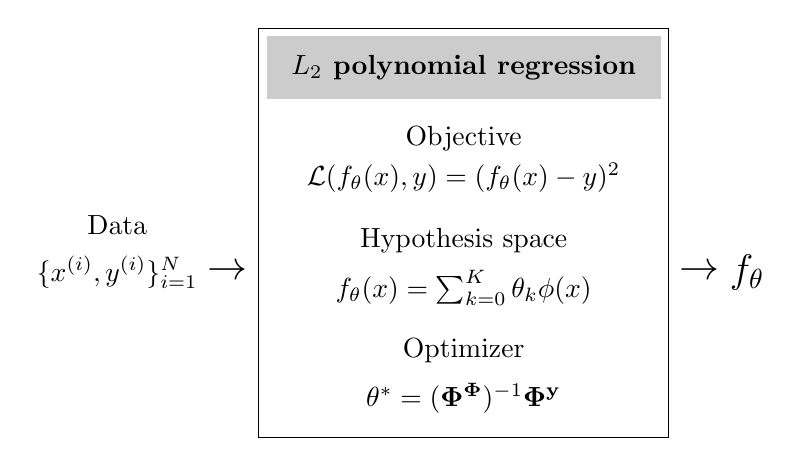
\begin{tikzpicture}
    \draw (0,0) rectangle (5.2,5.2); % outer box
    \fill[black!20] (0.1,4.3) rectangle (5.1,5.1); % gray box
    \node[] at (2.6,4.7) {{\bf $L_2$ polynomial regression}};
    \node[] at (2.6,3.8) {Objective}; \node[] at (2.6,3.3) {$\mathcal{L}(f_{\theta}(x),y) = (f_{\theta}(x)-y)^2$};
    \node[] at (2.6,2.5) {Hypothesis space}; \node[] at (2.6,1.9) {$f_{\theta}(x) = \sum_{k=0}^K \theta_k \phi(x)$};
    \node[] at (2.6,1.1) {Optimizer}; \node[] at (2.6,0.5) {$\theta^* = (\mathbf{\Phi}^\transpose\mathbf{\Phi})^{-1}\mathbf{\Phi}^\transpose\mathbf{y}$};
    \node[] at (-1.8,2.7) {Data};
    \node[] at (-1.8,2.1) {$\{x^{(i)}, y^{(i)}\}_{i=1}^N$};
    \node[] at (-0.4,2.1) {{\Large  $ \rightarrow$}};
    \node[] at (6.2,2.1) {{\Large $f_{\theta}$}};
    \node[] at (5.6,2.1) {{\Large  $ \rightarrow$}};
\end{tikzpicture}
\end{center}

% \begin{figure}[h]
%     \centering
%     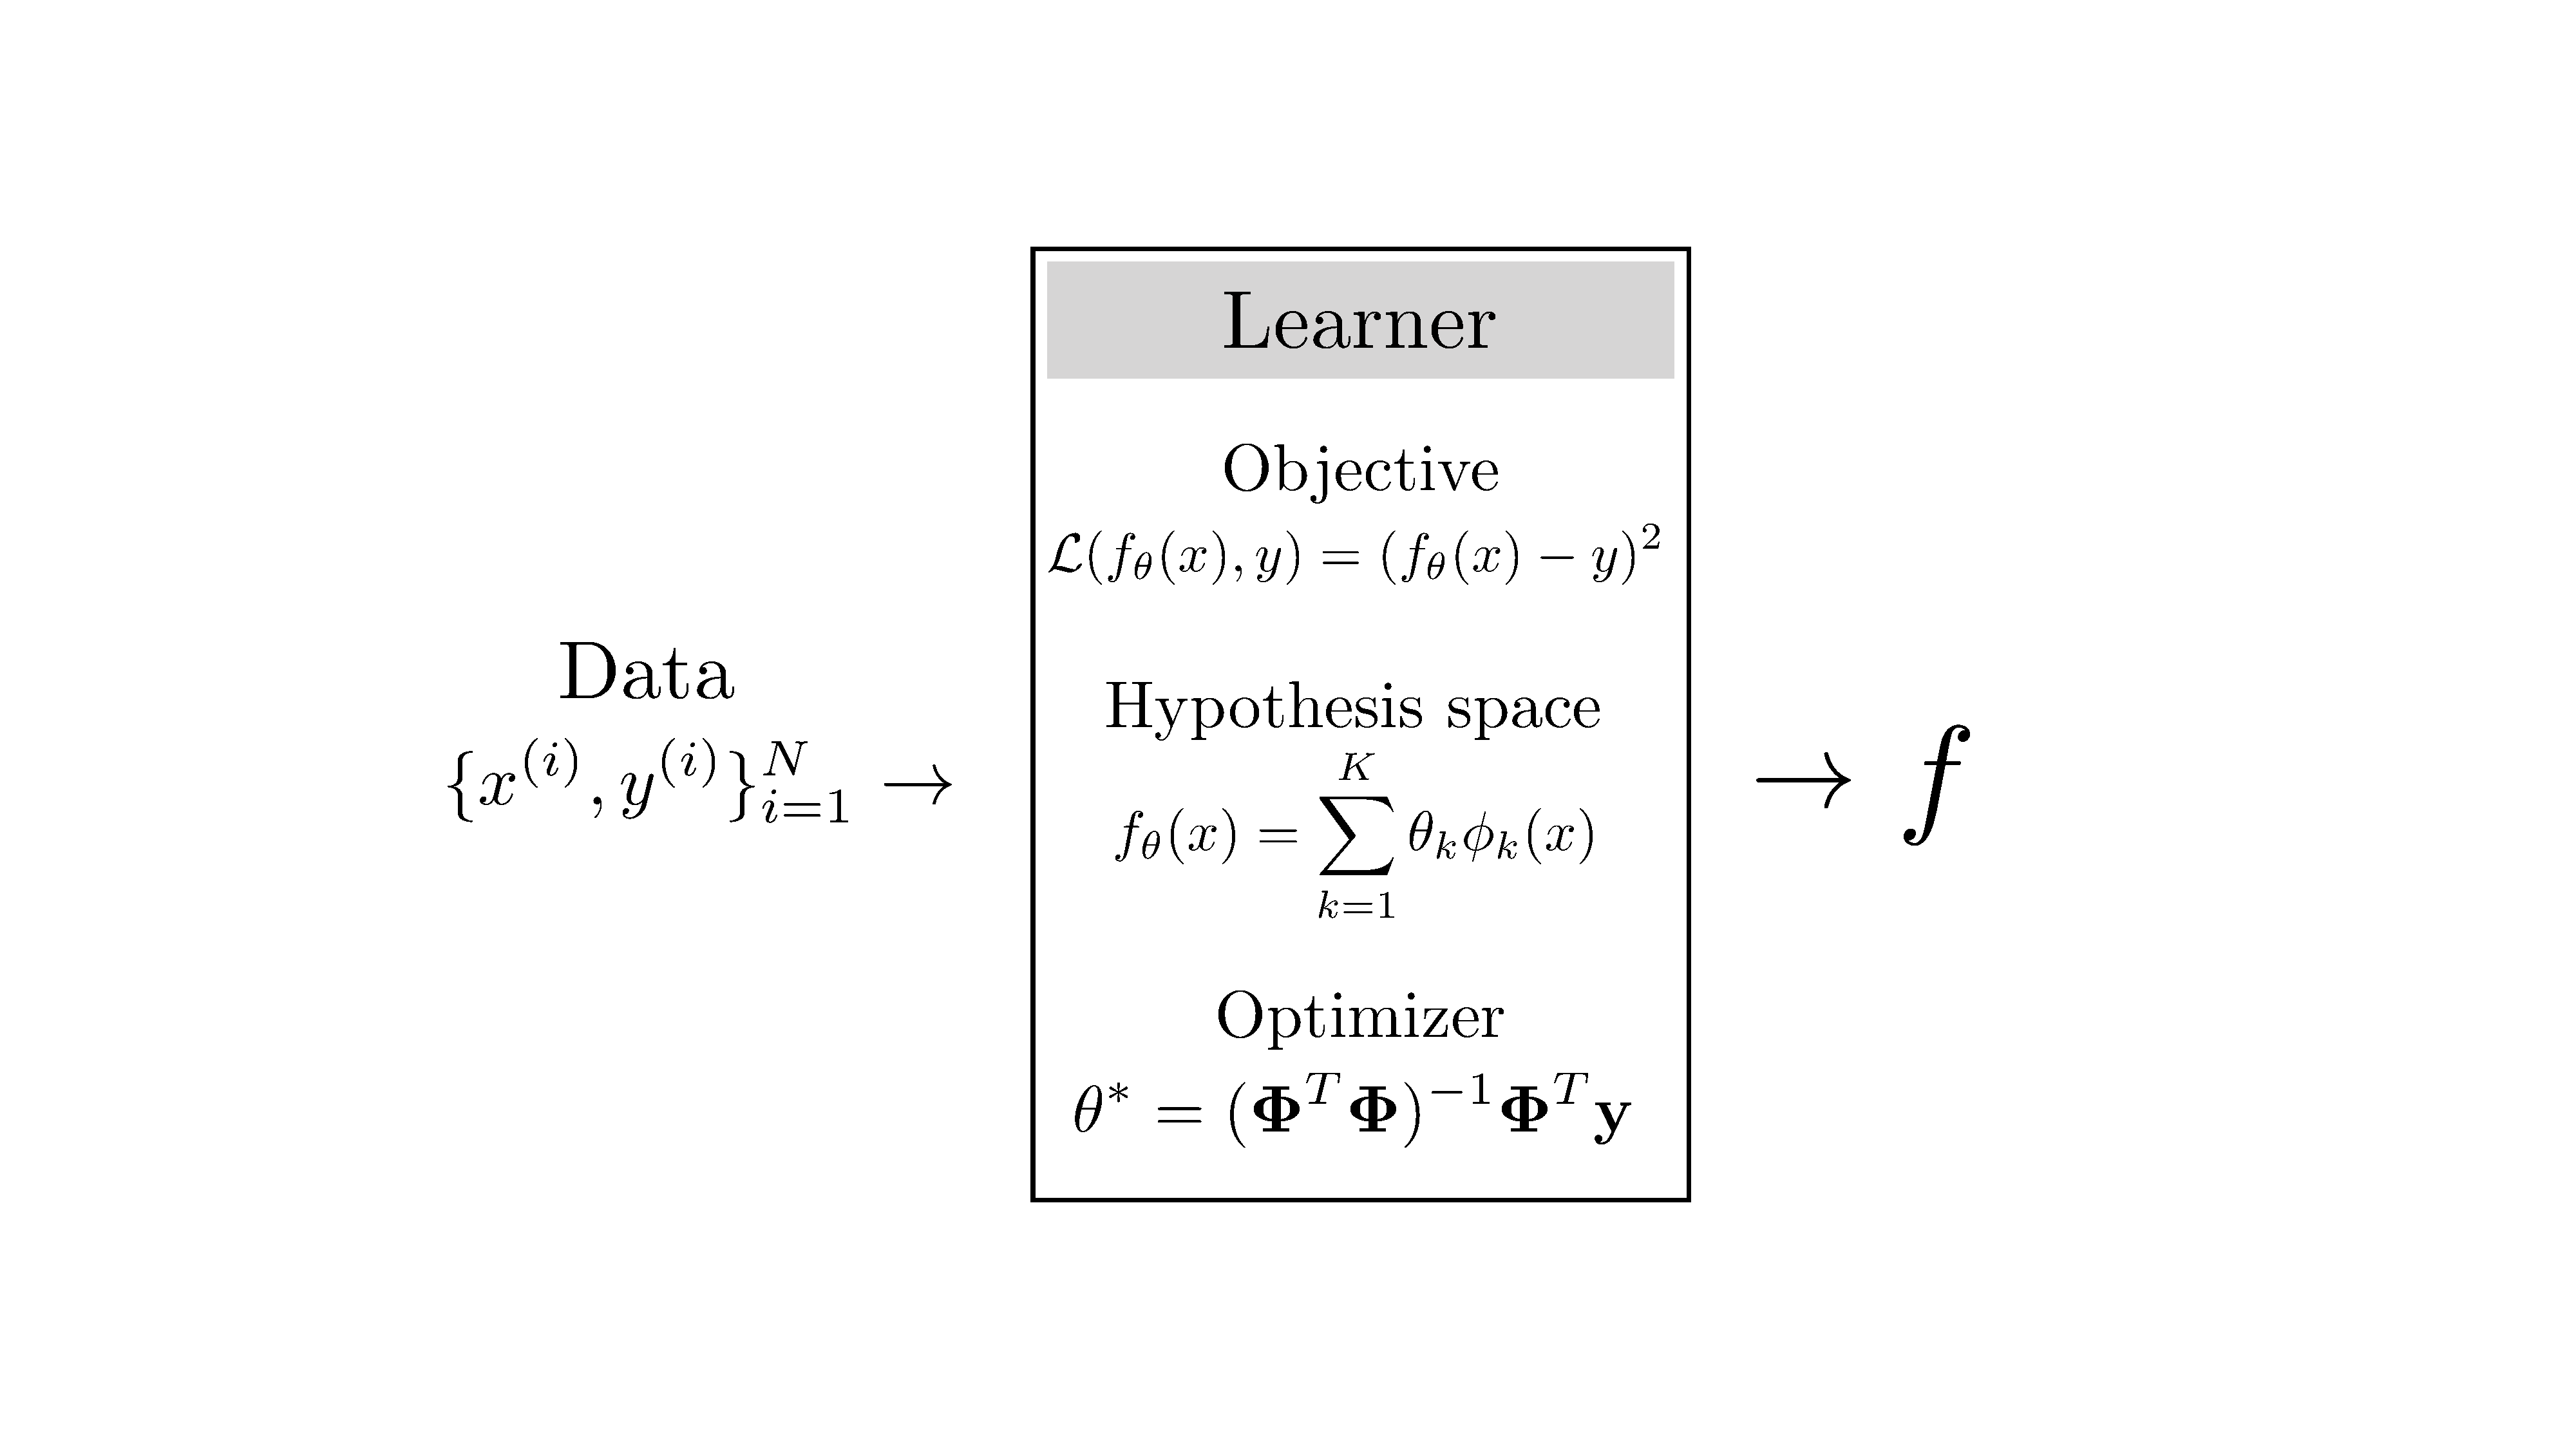
\includegraphics[width=0.65\linewidth]{./figures/problem_of_generalization/least_squares_polynomial_regression.pdf}
%     \label{fig:least_squares_polynomial_regression}
% \end{figure}

where
\begin{equation}
    \mathbf{\Phi} = 
     \begin{bmatrix}
        1 & x^{(1)} & x^{(1)^2} & ... & x^{(1)^K} \\
        1 & x^{(2)} & x^{(2)^2} & ... & x^{(2)^K} \\
        \vdots & \vdots & \vdots & \vdots & \vdots \\
        1 & x^{(N)} & x^{(N)^2} & ... & x^{(N)^K}  \\
    \end{bmatrix}
\end{equation}
\marginnote{This same trick works for any kind of function $\phi$, not just polynomials. The $\phi$ could be an expansion into a Fourier basis, for example. The general name for this kind of regression is {\bf basis function regression}; it is equivalent to linear regression on top of \textit{features} of $x$ (i.e., functions of $x$) rather than directly on $x$ itself.}[-6cm]

The matrix $\mathbf{\Phi}$ is an array of the features (columns) for each datapoint (rows). It plays the same role as data matrix $\mathbf{X}$ did in \chap{\ref{chapter:intro_to_learning}}; in fact we often call matrices of the feature representations of each datapoint also as a \textbf{data matrix}. As an exercise, you can derive the closed form of the optimizer, given above, using the same steps as we did for linear regression in \chap{\ref{chapter:intro_to_learning}}.\marginnote{When we get to the chapters on neural nets we will see that data matrices appear all over. A neural net is a sequence of transformations of an input data matrix into increasingly more powerful feature representations of the data, i.e. a sequence of better and better data matrices.}[-4.3cm]

\subsection{Polynomial Regression as a Lens into Generalization}
%To understand underfitting we measure it with {\bf approximation error}. The latter is called overfitting and we measure it with {\bf generalization error}.

What happens as we increase the order of the polynomial $K$, that is, we use $K+1$ basis functions $x^0, \ldots, x^K$? With $K=1$, we arrive back at linear regression. With $K=2$, we are fitting quadratic functions (i.e., parabolas) to the training data. As $K$ increases, the hypothesis space expands to include ever more curvy fits to the data, as shown in \fig{\ref{fig:under_and_overfitting}}.

\begin{figure}[h]
    \centerline{
    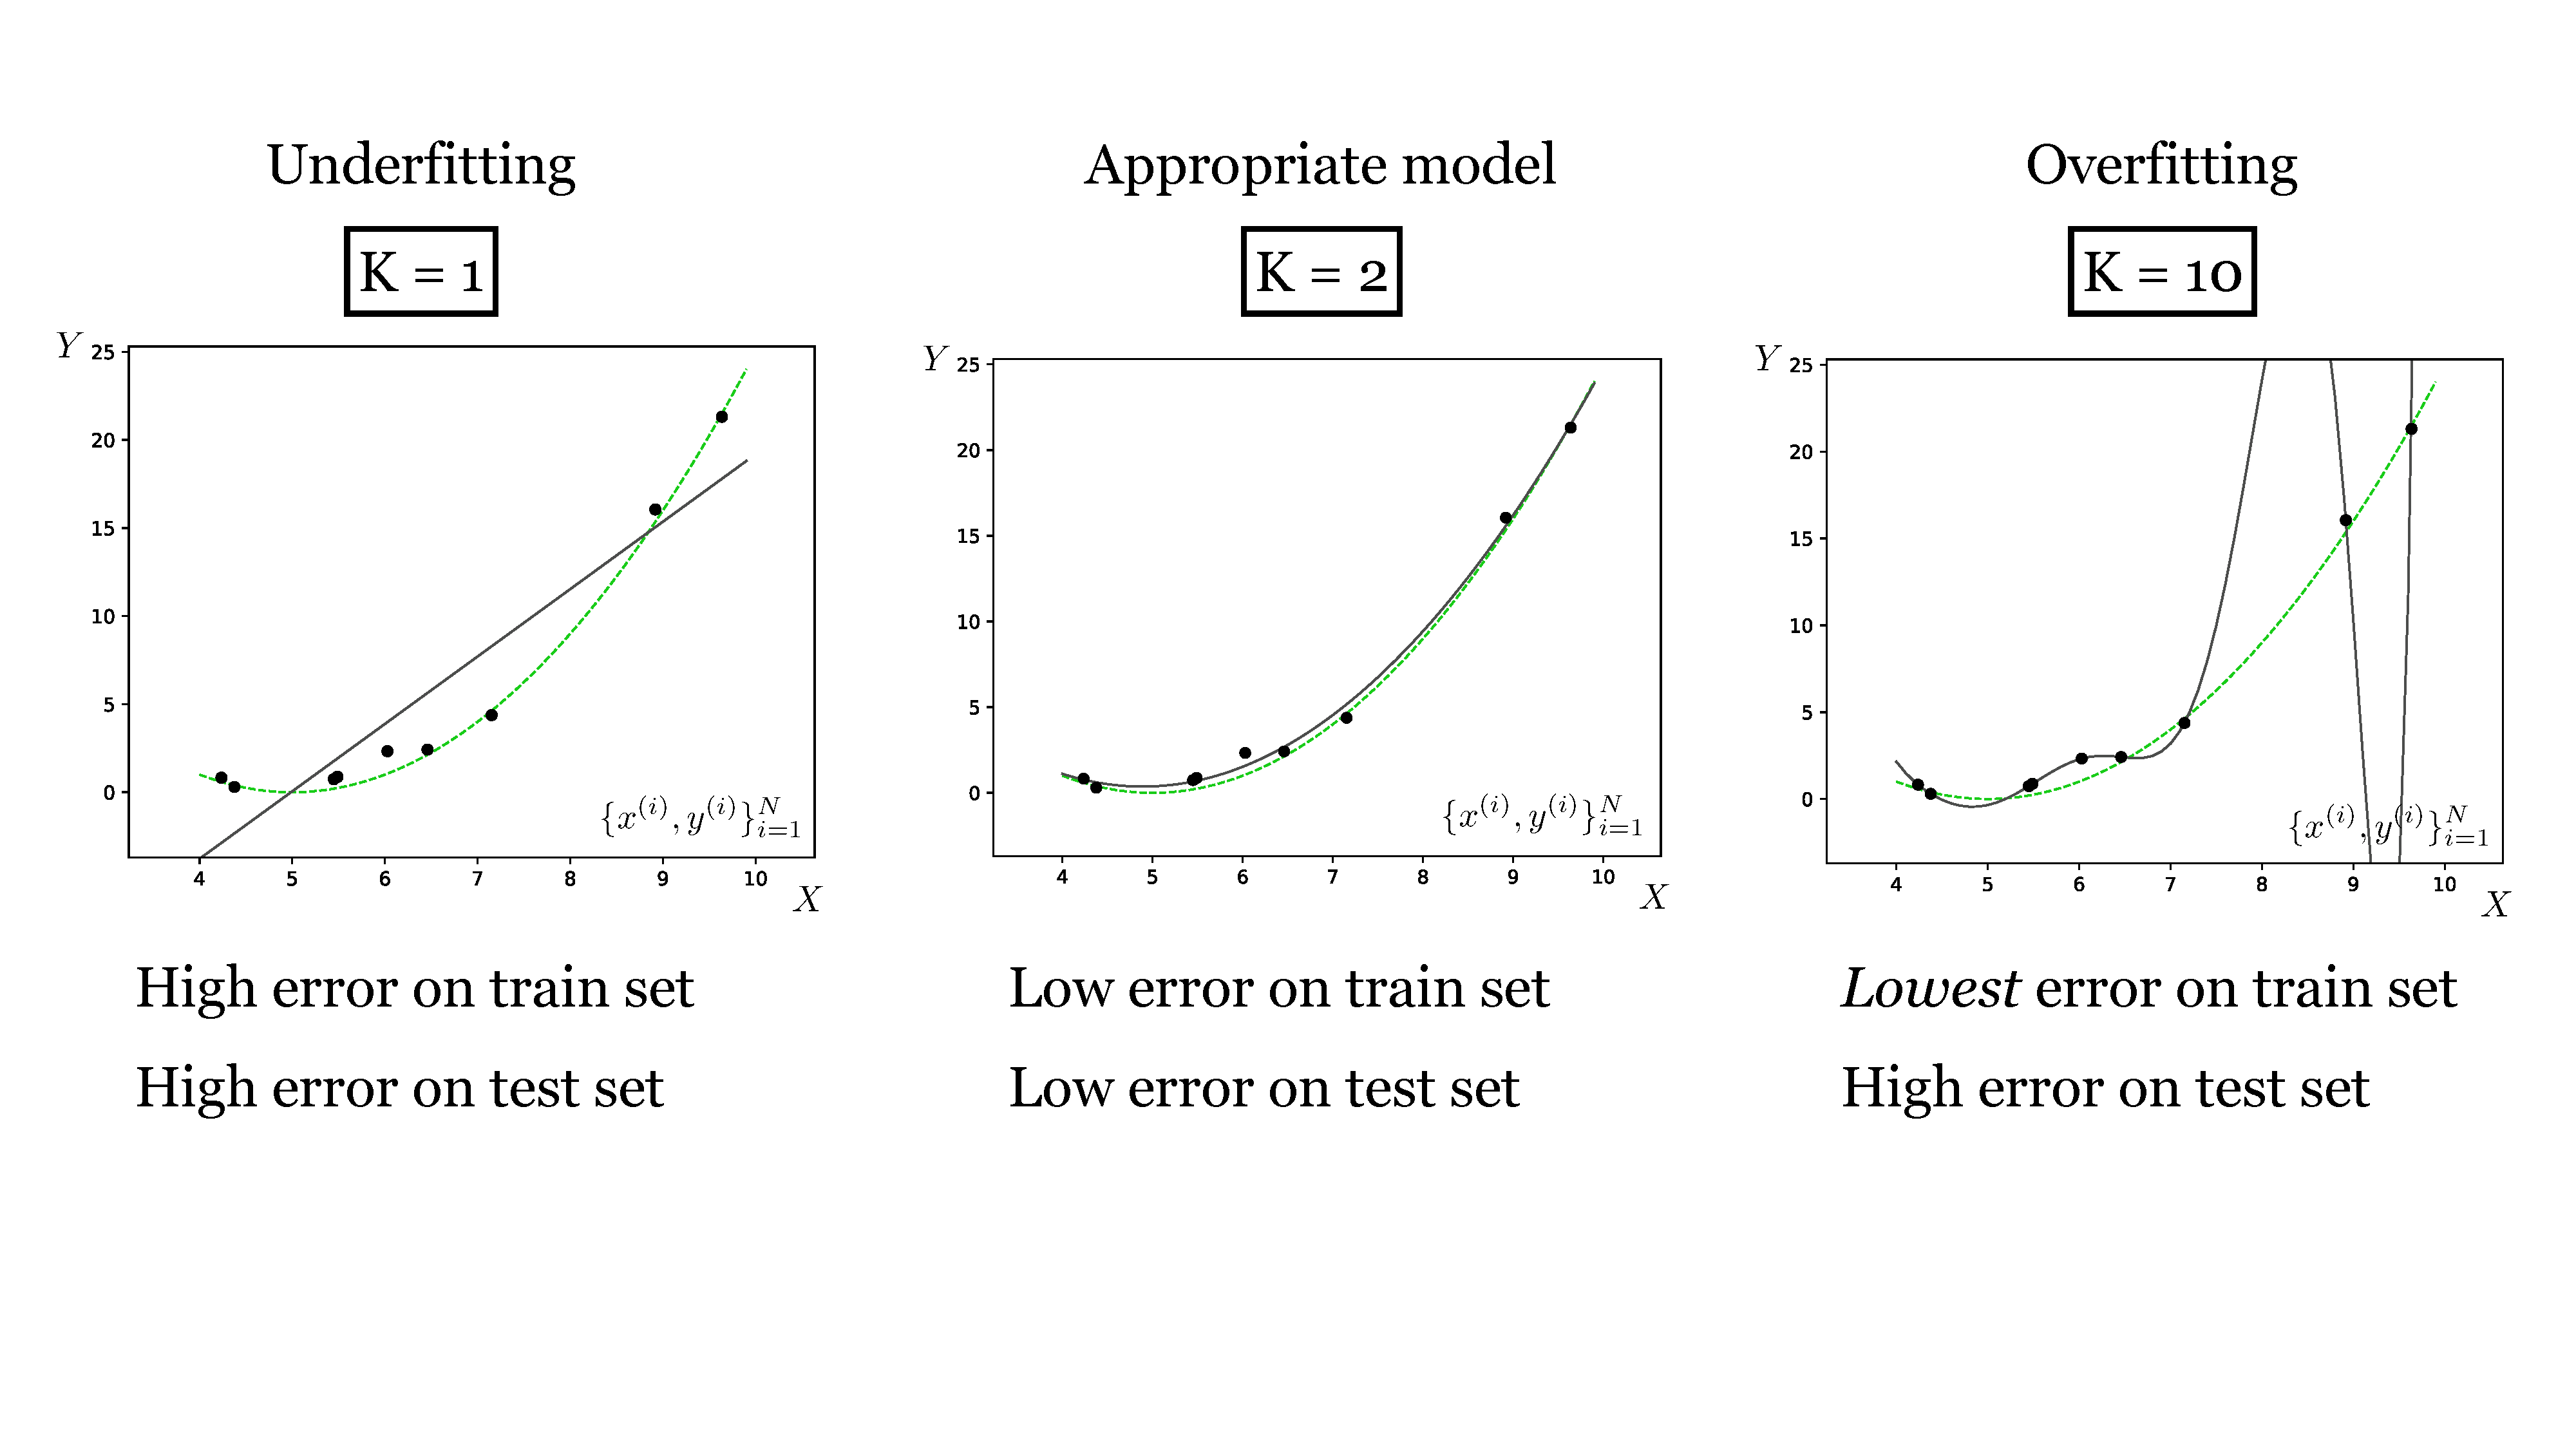
\includegraphics[width=1.0\linewidth]{./figures/problem_of_generalization/under_and_overfitting.pdf}
    }
    \caption{Underfitting and overfitting.}
    \label{fig:under_and_overfitting}
\end{figure}

The black line is the model's fit. The green line is the ground truth relationship between random variables $X$ and $Y$. The observed data $\{x^{(i)}, y^{(i)}\}_{i=1}^N$ is the black points, and this data is sampled from the green line plus observation noise. We refer to the full process that generates the data as the {\bf data generating process}:
\begin{align}
    Y &= X^2 + 1 &\triangleleft \quad\text{true underlying relationship}\\
    \epsilon &\sim \mathcal{N}(0,1) &\triangleleft \quad\text{observation noise}\\
    Y^\prime &= Y + \epsilon &\triangleleft \quad\text{noisy observations}\\
    x,y &\sim p(X,Y^{\prime}) &\triangleleft \quad\text{data-generating process}
\end{align}\marginnote{This data generating process assumes there is no noise in our observations of $x$. This is a common assumption in least-squares regression problems. Other models relax this assumption; for example, the generative models we will see in \chap{\ref{chapter:generative_models}} model uncertainty in both the $x$ and $y$ observations jointly.}[-3cm]
As we increase $K$ we fit the data points better and better, but eventually start \emph{overfitting}, where the model perfectly interpolates the data (passes through every datapoint) but deviates more and more from the true data-generating line. Why does that happen? It's because for $K=10$ the curve can become wiggly enough to not just fit the true underlying relationship but also to \textit{fit the noise}, the minor offsets $\epsilon$ around the green line. This noise is \textit{a property of the training data that does not generalize to the test data}; the test data will have different observation noise. That's what we mean when we say a model is overfitting.

As $K$ grows, a second phenomenon also occurs. For $K=10$ there are many hypotheses (polynomial functions) that perfectly the data (true function + noise) -- there is insufficient data for the objective to uniquely identify one of the hypotheses to be the best. Because of this, the hypothesis output by the optimizer may be an arbitrary one, or rather will be due to details of the optimization algorithm (e.g., how it is initialized), rather than selected by the objective. The optimizer we used above has a tendency to pick, among all the equally good hypotheses, one that is very curvy. This is an especially bad choice in this example, because the true function is much more smooth.

%So, overfitting can include two phenomena (both of which we see here): the model can be fitting noise (aspects of training data that don't generalize to test data) and the model might be underconstrained, having no unique minimizer to the objective, and therefore 

\index{Approximation error}{\bf Approximation error} is the gap between the black line and the training data points. Let $\{x_{(\texttt{train})}^{(i)}, y_{(\texttt{train})}^{(i)}\}_{i=1}^N$ be our training data set (the black points). Then the approximation error $J_{\texttt{approx}}$ is defined as the total cost incurred on this training data:
\begin{align}
    J_{\texttt{approx}} = \frac{1}{N} \sum_{i=1}^N \mathcal{L}(f_{\theta}(x_{(\texttt{train})}^{(i)}), y_{(\texttt{train})}^{(i)})
\end{align}
Notice that approximation error is the cost function we minimize in empirical risk minimization (\chap{\ref{chapter:intro_to_learning}}).

\index{Generalization error}{\bf Generalization error} is the gap between the black line and the green line, that is, the expected cost we would incur if we sampled a new test point at random from the true data generating process. Generalization error is often approximated by measuring performance on a heldout \index{Validation dataset}{\bf validation dataset}, $\{x_{(\texttt{val})}^{(i)}, y_{(\texttt{val})}^{(i)}\}_{i=1}^N$, which can simply be a subset of the data that we don't use for training or testing:
\begin{align}
    J_{\texttt{gen}} &= \mathbb{E}_{x,y \sim p_{\texttt{data}}} [ \mathcal{L}(f_{\theta}(x), y)]\\
                        &\approx \frac{1}{N} \sum_{i=1}^N \mathcal{L}(f_{\theta}(x_{(\texttt{val})}^{(i)}), y_{(\texttt{val})}^{(i)})
\end{align}

Approximation error goes down with increasing $K$ but all we really care about is generalization error, which measures how well we will do on test queries that are newly sampled from the true data generating process. For polynomial regression, generalization error obeys a U-shaped function with respect to $K$: at first it is high because we are underfitting; gradually we fit the data better and better and eventually we overfit, with generalization error becoming high again. \Fig{\ref{fig:under_and_overfitting_vs_polyK}} shows how it looks like for our example.
\begin{figure}[h]
    \centerline{
    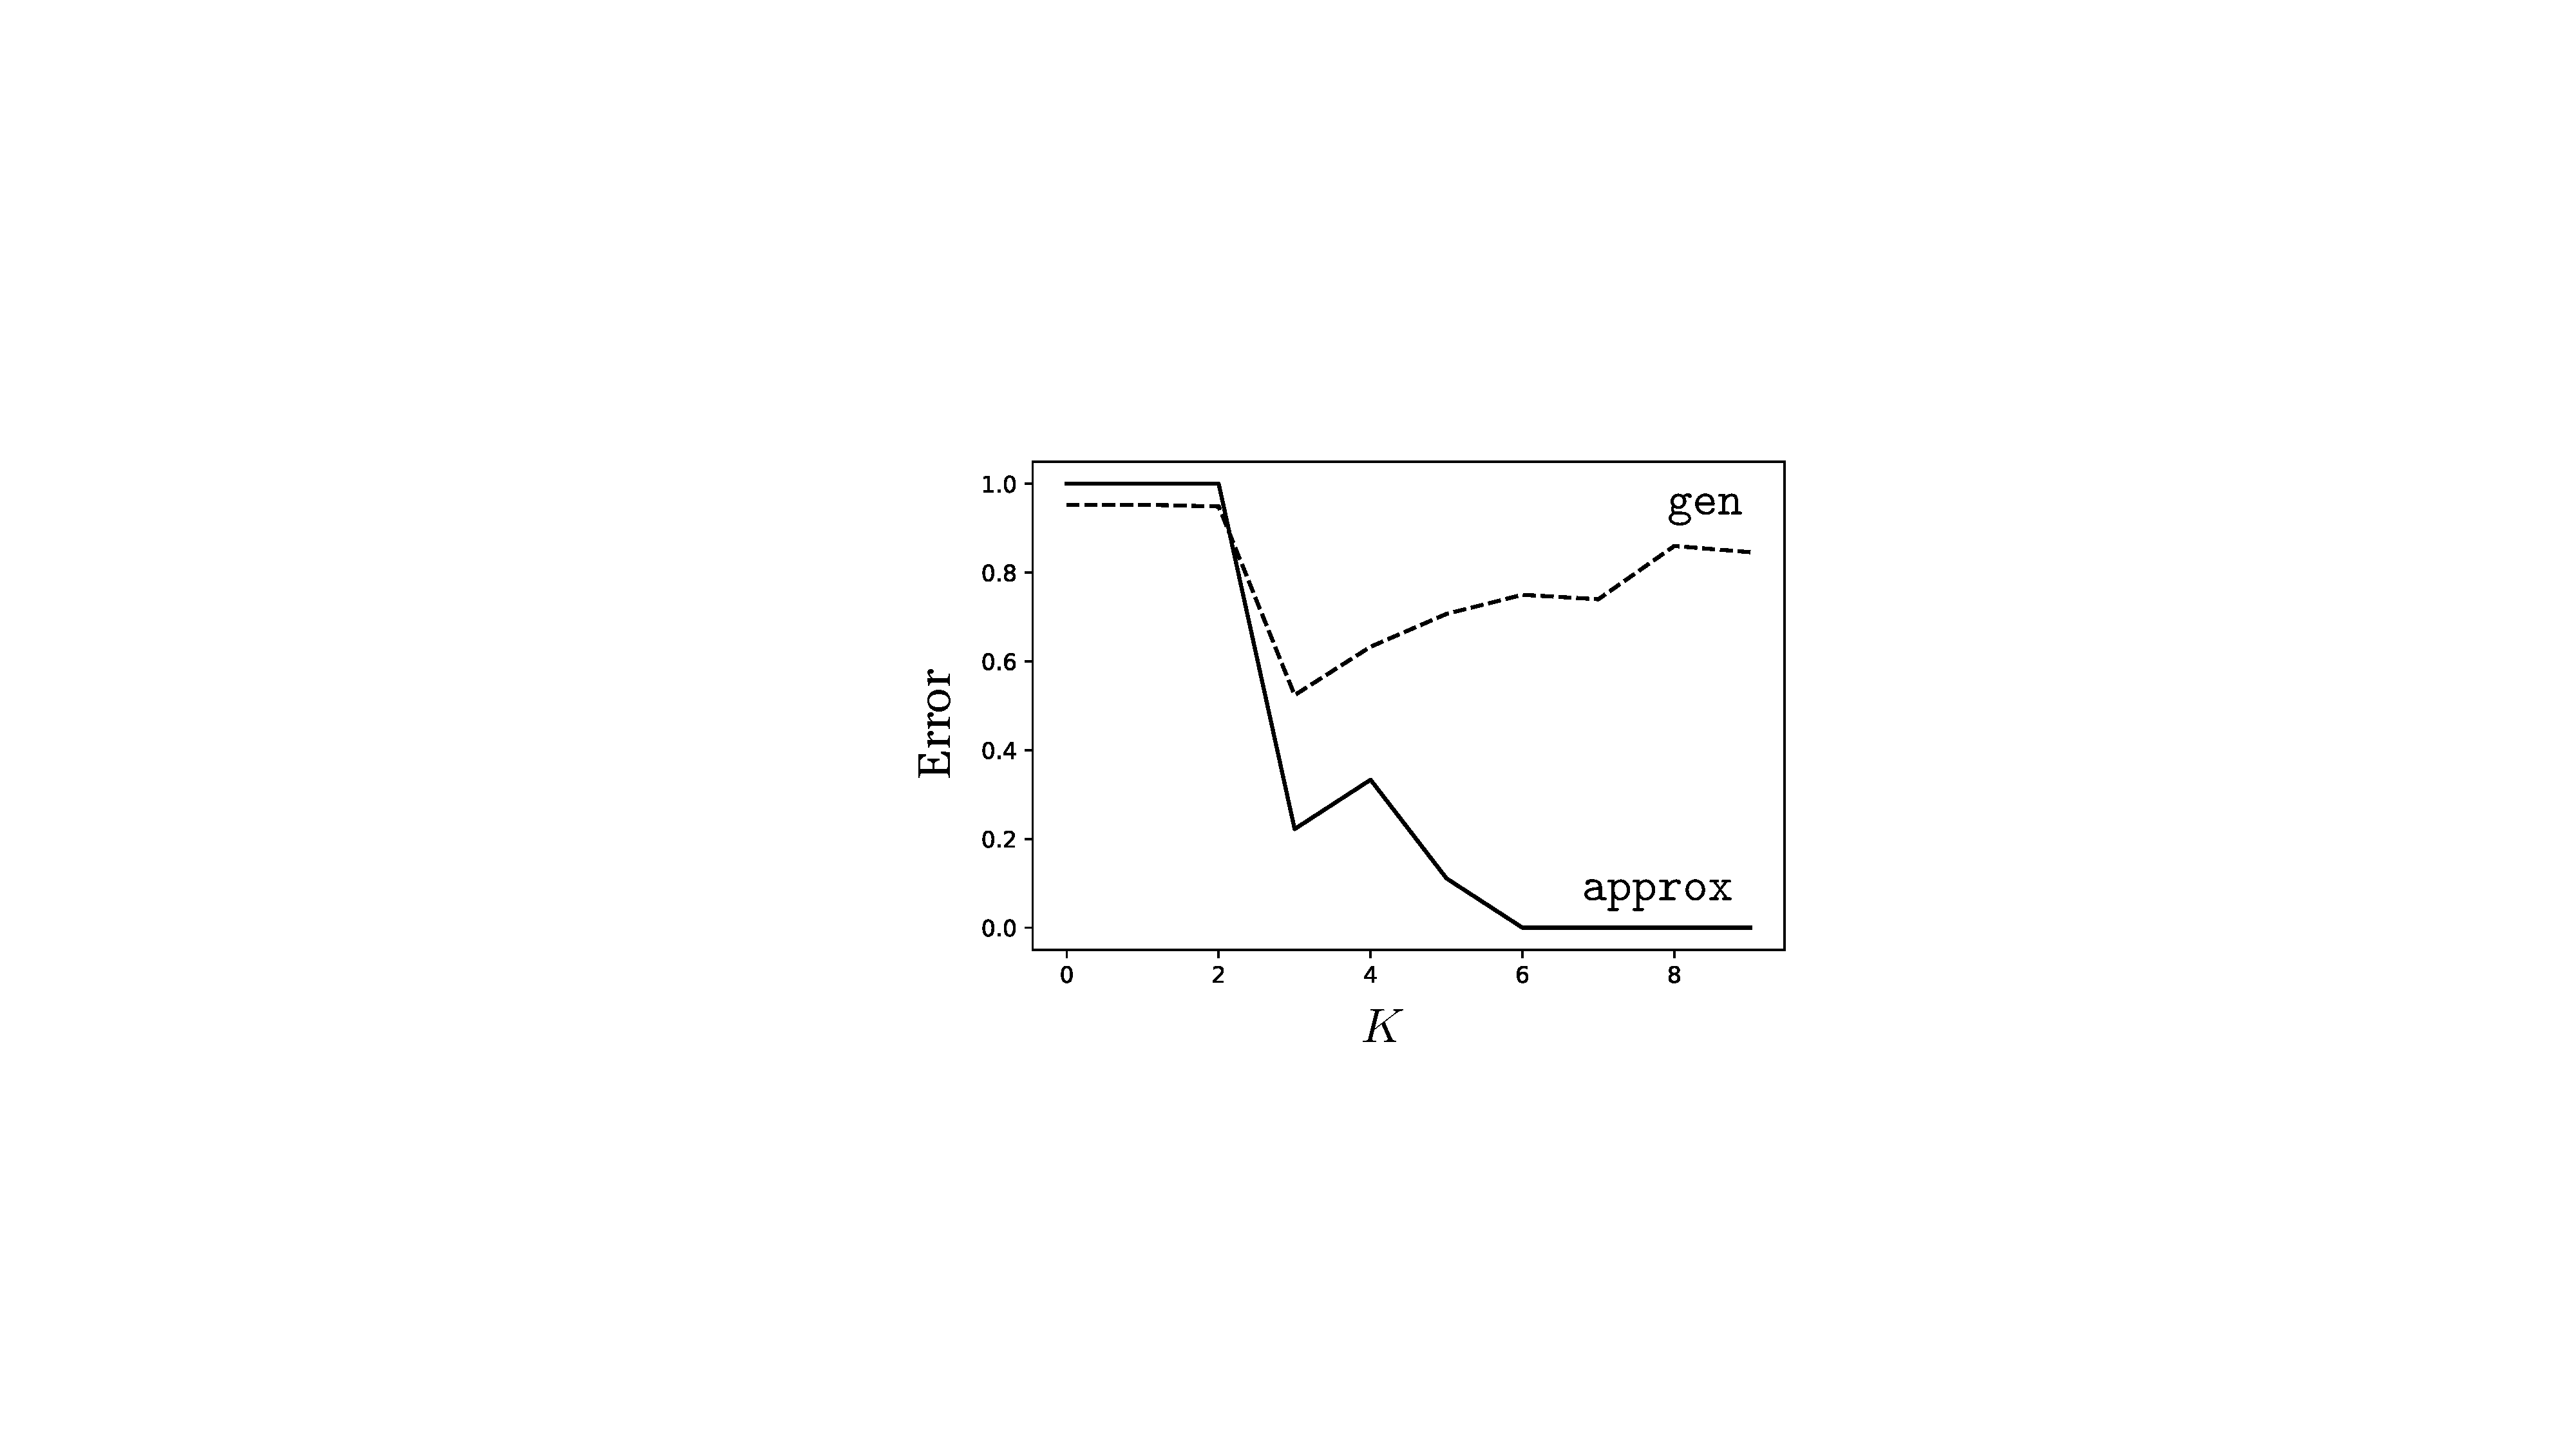
\includegraphics[width=0.48\linewidth]{./figures/problem_of_generalization/under_and_overfitting_vs_polyK.pdf}
    }
    \caption{Approximation error (\texttt{approx}) versus generalization error (\texttt{gen}) for polynomial regression of order $K$. Here we measured error as the proportion of validation points that are mispredicted (defined as having an $L_2$ prediction error greater than 0.25).}
    \label{fig:under_and_overfitting_vs_polyK}
\end{figure} %We use this notion of error since if we plotted the cost $J_{\texttt{gen}}$ as a function of $K$, for high values of $K$ the error becomes so large that the plot looks like a hockey stick and we only get to see one side of the U-shape.}[2.5cm]

This U-shaped curve is characteristic of classical learning regimes like polynomial regression, where we often find that the more parameters a model has, the more it will tend to overfit. However, this behavior does not well characterize modern learners like deep neural networks. Deep networks, which we will see in \chap{\ref{chapter:neural_nets}}, can indeed either underfit or overfit, but it is not the case that there is a simple relationship between the number of parameters the net has and whether that leads to underfitting versus overfitting. In fact, bigger deep nets with more parameters may overfit less than smaller nets. We discuss this further in \sect{\ref{sect:problem_of_generalization:rethinking_generalization}}. 

%\section{Bias-variance tradeoff}

%This idea can be formalized via the {\bf bias-variance tradeoff}.

%Show empirical plot from DLAICV. 

%An important concept in learning theory is {\bf model capacity}. 


\section{Regularization}

The previous example suggests a kind of ``Goldilocks principle.'' We should prefer hypotheses (functions $f$) that are sufficiently expressive to fit the data, but not so flexible that they can overfit the data. 


\index{Regularization}{\bf Regularization} refers to mechanisms that penalize function complexity so that we avoid learning too flexible a function that overfits. 
%Model capacity measures the expressivity of the hypothesis space. 
Typically, regularizers are terms we add to the objective that prefer simple functions in the hypothesis space, all else being equal. They therefore embody the principle of \index{Occam's razor}{\bf Occam's razor}. The general form of a regularized objective is:
\begin{align}
    J(\theta) = \overbrace{\frac{1}{N} \sum^N_{i=1} \mathcal{L}(f_{\theta}(x)^{(i)}, y^{(i)})}^\text{data fit loss} + \underbrace{\lambda R(\theta)}_\text{regularizer} \quad\quad\triangleleft \quad\text{regularized objective function} \label{eqn:problem_of_generalization:regularized_objective}
\end{align}
where $\lambda$ is a hyperparameter that controls the strength of the regularization.

One of the most common regularizers is to penalize the $L_p$ norm of the parameters of our model, $\theta$:
\begin{equation}
    R(\theta) = \norm{\theta}_{p}.
\end{equation}
\marginnote{The $L_p$-norm of $\mathbf{x}$ is $(\sum_i |x_i|^{p})^{\frac{1}{p}}$. The $L_2$-norm is the familiar least-squares objective.}[-0.4cm]
An especially common choice is $p=2$, in which case the regularizer is called \index{Ridge regression}{\bf ridge regularization} (which is also known as {\bf Tikonov regression}). In the context of neural networks, this regularizer is called \index{Weight decay}{\bf weight decay}. When $p=1$, the regularizer, applied to regression problems, is called \index{LASSO regression}{\bf LASSO regression}. For any $p$, the effect is to encourage most parameters to be zero, or near zero. When most parameters are zero, the function takes on a degenerate form, that is, a simpler form. For example, if we consider the quadratic hypothesis space $\theta_1 x + \theta_2 x^2$, then, if we use a strong $L_p$ regularizer, and if a linear fit is almost perfect, then $\theta_2$ will be forced to zero and the learned function will be linear rather than quadratic. Again, we find that regularization is an embodiment of Occam's razor: when multiple functions can explain the data, give preference to the simplest.

\subsection{Regularizers as Probabilistic Priors} Regularizers can be interpreted as \index{Priors}\textbf{priors} that prefer, a priori (before looking at the data), some solutions over others. Under this interpretation, the data fit loss (e.g., $L_2$ loss) is a likelihood function $p(\{y^{(i)}\}^N_{i=1} \given \{x^{(i)}\}^N_{i=1}, \theta)$ and the regularizer is a prior $p(\theta)$. Bayes' rule then states that the posterior $p(\theta \given \{x^{(i)}, y^{(i)}\}^N_{i=1})$ is proportional to the product of the prior and the likelihood. The log posterior is then the \textit{sum} of the log likelihood and the log prior, plus a constant. Hence we arrive at the form of \eqn{\ref{eqn:problem_of_generalization:regularized_objective}}.

\subsection{Revisiting the $\star$ Problem}\label{sec:problem_of_generalization:star_problem_revisited}
Remember the $\star$ problem from \chap{\ref{chapter:intro_to_learning}}?
\begin{align}
    3 \star 2 &= 36\nonumber \\
    7 \star 1 &= 49\nonumber \\
    5 \star 2 &= 100\nonumber \\
    2 \star 2 &= 16\nonumber
\end{align}
You may have figured out that $x \star y = (xy)^2$. We said that is the correct answer. But hold on, couldn't it be that $x \star y =  94.5x - 9.5x^2 + 4y^2 - 151$? That also perfectly explains these four examples (trust us, we checked). Or maybe $\star$ is the following Python program (\fig{\ref{fig:problem_of_generalization:python_star_solution}}).
\begin{figure}[h]
\begin{minipage}{1.0\linewidth}
\begin{minted}[xleftmargin=0.33\linewidth,xrightmargin=0.33\linewidth,
fontsize=\fontsize{8.5}{9},
frame=single,
framesep=2.5pt,
baselinestretch=1.05,
]{python}
def star(x,y):
    if x==2 && y==3:
        return 36
    elif x==7 && y==1:
        return 49
    elif x==5 && y==2:
        return 100
    elif x==2 && y==2:
        return 16
    else:
        return 0
\end{minted}
\end{minipage}
%}
\caption{A function written in Python that solves the $\star$ problem from \chap{\ref{chapter:intro_to_learning}}.}
\label{fig:problem_of_generalization:python_star_solution}
\end{figure}

That also perfectly fits the observed data. Why didn't you come up with those answers? What made $x \star y = (xy)^2$ more compelling?

We suspect your reason is again Occam's razor, which states that when multiple hypotheses equally well fit the data, you should prefer the simplest. To a human, it may be that $x \star y = (xy)^2$ is the simplest. To a computer, defining a proper notion of simplicity is a hard problem, but can be made precise.

As we saw, most regularizers can be given probabilistic interpretations as priors on the hypothesis, whereas the original objective (e.g., least-squares) measures the likelihood of the data given the hypothesis. These priors are not arbitrarily chosen. The notion of the {\bf Bayesian Occam's razor} derives such priors by noting that more complex hypothesis spaces must cover more possible hypotheses, and therefore must assign less prior mass to any single hypothesis (the prior probability of all possible hypotheses in the hypothesis space must sum to 1)~\cite{jefferys1992ockham, mackay2003information}. This is why, probabilistically, simpler hypotheses are more likely to be true.

\section{Rethinking Generalization} \label{sect:problem_of_generalization:rethinking_generalization}
A recent empirical finding is that some seemingly complex hypothesis spaces, such as deep nets (which we will see in later chapters), tend not to overfit, even though they have many more free parameters than the number of datapoints they are fit to. Exactly why this happens is an ongoing topic of research~\cite{zhang2016understanding}. But we should not be too surprised. The number of parameters is just a rough proxy for model capacity (i.e., the expressivity of the hypothesis space). A single parameter that has infinite numerical precision can parameterize an arbitrarily complex function. Such a parameter defines a very expressive hypothesis space and will be capable of overfitting data. Conversely, if we have a million parameters, but they are regularized so that almost all are zero, then these parameters may end up defining a simple class of functions, which does not overfit the data. So you can think of the number of parameters as a rough estimate of model capacity, but it is not at all the full story. See \cite{belkin2018reconciling} for more discussion on this point.%Overfitting is fundamentally related to \emph{model capacity}, not number of parameters, but often number of parameters is a good proxy. %Ideas from information theory can be used to define more appropriate measures of expressivity than ``number of parameters". %However, it has long been clear that overfitting is not really about \emph{number} of free parameters, rather the complexity of the hypothesis space. A function with many parameters tends to be more complex than a function with   

\section{Three Tools in the Search for Truth: Data, Priors, and Hypotheses}

In this section, we will introduce a perspective on learning and generalization that puts all our tools together. We will consider learning as akin to searching for the proverbial needle in a haystack. The haystack is our search space (i.e., the hypothesis space). The needle is the ``truth'' we are seeking, that is, the true function that generates our observations. 

We have several tools at our disposal to help us pinpoint the location of the needle, and in this section we will focus on the following three: \textit{data}, \textit{priors}, and \textit{hypotheses}. 

The first tool, \textit{data}, was the topic of \chap{\ref{chapter:intro_to_learning}}. In vision, the data is observations of the world like photos and videos. Finding explanations consistent with the observed data is the centerpiece of learning-based vision.

The second tool at our disposal was introduced earlier in this chapter: priors (a.k.a. regularizers) that prefer some solutions over others a priori. 

The last tool at our disposal is the set of \textit{hypotheses} under consideration for what the true function may be. The hypothesis space constrains which solutions we can possibly find. If the true solution is not in our hypothesis space, then no amount of data or priors can help us find it. This situation is like the old joke of a drunk man looking for his lost keys under a lamppost~\cite{freedman2010wrong}. ``Why are you looking there,'' a cop asks. ``Because this is where the light is.''

Together these three tools allow us to pinpoint one (or a few) good solutions in the space of all possibilities, as depicted in the cartoon in \fig{\ref{fig:problem_of_generalization:search_space_tools}}.
%\vspace{-0.3cm}

In this cartoon, we are learning a mapping from some domain $\mathcal{X}$ to another domain $\mathcal{Y}$. The hypothesis space, $\mathcal{F}$ (white circle; ``the lamppost's light'') places a hard constraint on the subset of possible mappings under consideration, the prior (yellow ellipse) places a soft constraint on which mappings are preferred over which others, and the data (green ellipse) also places a soft constraint on the space, preferring mappings that well fit the data. 

\begin{figure}[t]
    \centerline{
    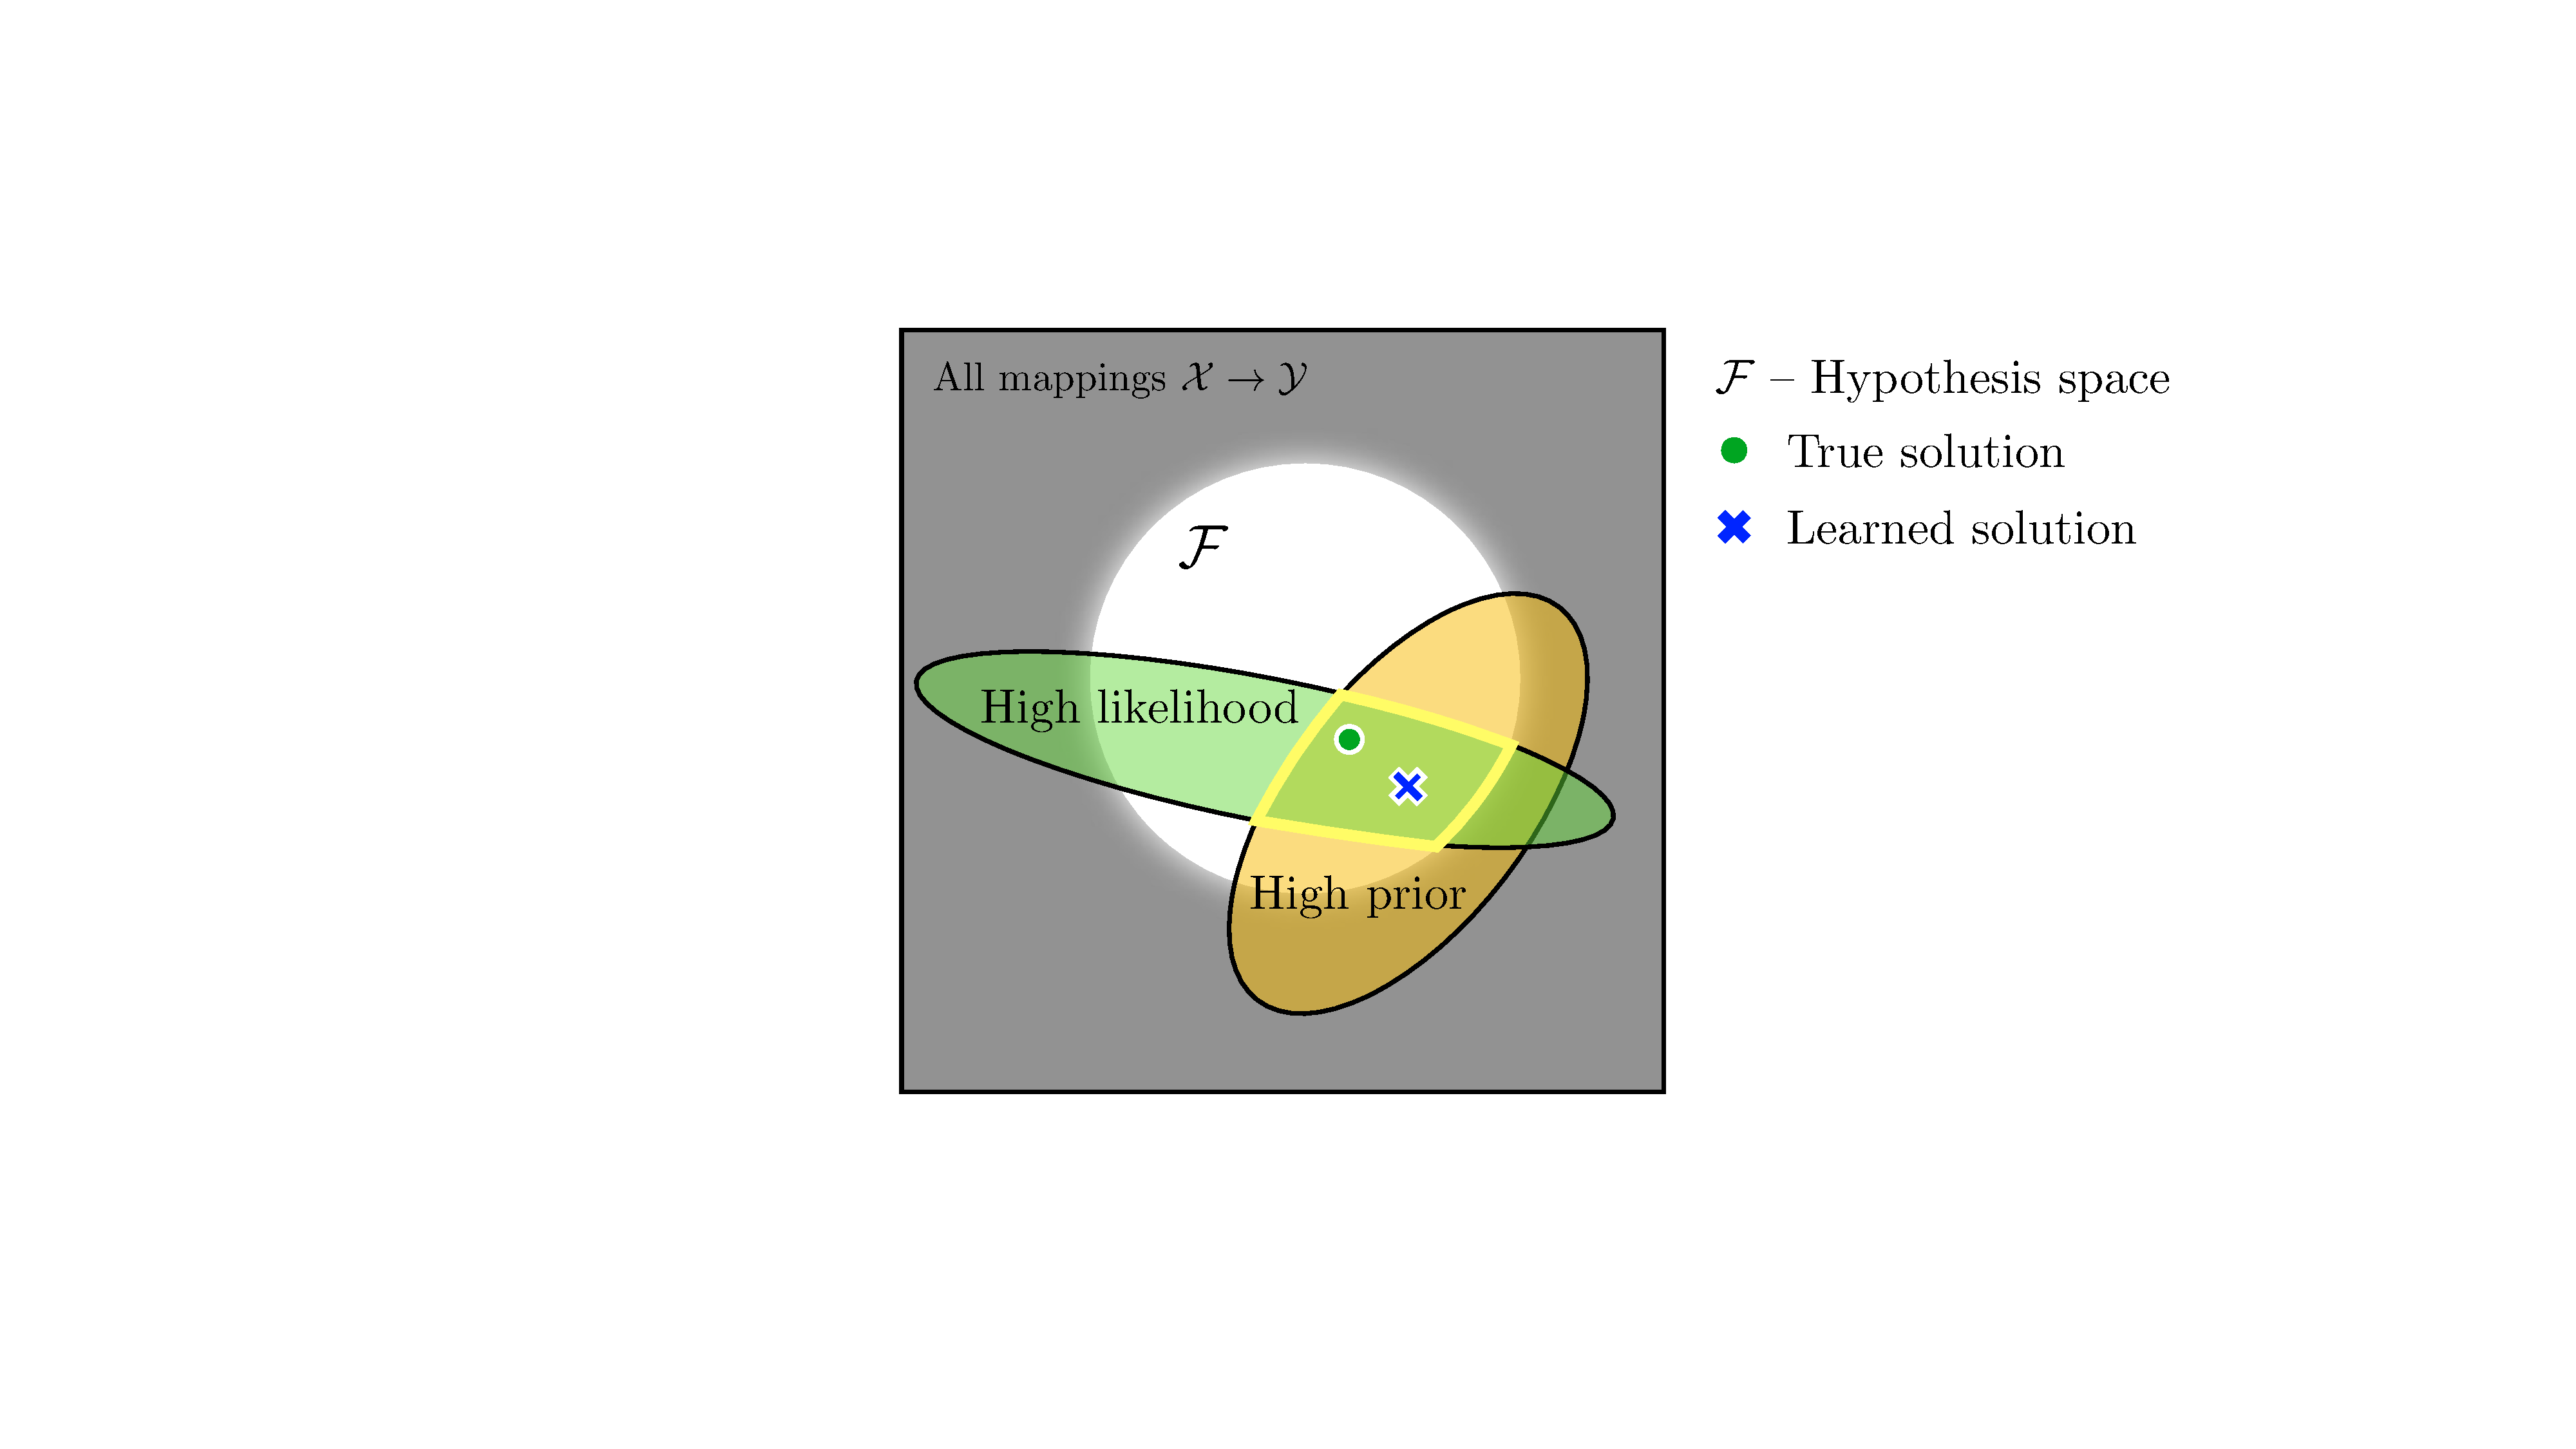
\includegraphics[width=0.65\linewidth]{./figures/problem_of_generalization/search_space_tools.pdf}
    }
    \caption{A cartoon of the tools for honing in on the truth.}
    \label{fig:problem_of_generalization:search_space_tools}
\end{figure}


Approximation error is low within the green region. If we didn't care about generalization, then it would be sufficient just to select any solution in this green region. But since we do care about generalization, we bias our picks toward the yellow region, which corresponds to a prior that selects points we believe to be closer to the true solution, even if they might not fit the data perfectly well. These tools isolate the area outlined in bright yellow as the region where we may find our needle of truth. A learning algorithm, which searches over $\mathcal{F}$ in order to maximize the likelihood times the prior, will find a solution somewhere in this outlined region. %The found solution will not necessarily coincide with the true solution but cannot be too far off, as long as the yellow outlined region indeed contains the truth. %will hopefully be nearby; if we shrink the yellow outlined region then we can be force the learner to get ever closer to the truth. 
%But it might not find the exact location of the true solution as the intersection of all our tools did not identify a unique solution in this example.

In the next three sections, we will explore these three tools in more detail through the simple experiment of fitting a curve to a set of datapoints.


\subsection{Experiment 1: Effect of Data}

Training data is the main source of information for a learner, and a learner is just like a detective: as it observes more and more data, it gets more and more evidence to narrow in on the solution. Here we will look at how data shapes the objective function $J$ for the following empirical risk minimization problem:
\begin{align}
    J(\theta; \{x^{(i)}, y^{(i)}\}^N_{i=1}) &= \frac{1}{N}\sum_i \lvert f_{\theta}(x^{(i)}) - y^{(i)}\rvert^{0.25} \quad\quad \triangleleft \quad\text{objective}\label{eqn:problem_of_generalization:error_fn_1}\\
    f_{\theta}(x) &= \theta_0 x + \theta_1 \sin(x)  \quad\quad \triangleleft \quad\text{hypothesis space}
\end{align}\marginnote{We use the exponent $0.25$, rather than the more common squared error, just so that the plots in \fig{\ref{fig:problem_of_generalization:more_data_more_constraints}} show more clearly the linear constraints (the dark lines) added by each datapoint to the objective $J$.}[-1.6cm]
In \fig{\ref{fig:problem_of_generalization:more_data_more_constraints}}, bottom row, we plot $J$ as a heatmap over the values obtained for different settings of $\theta$. On the top row we plot the data being fit, $\{x^{(i)}, y^{(i)}\}^N_{i=1}$, along with the function $f_{\theta}$ that achieves the best fit, and a sample other settings of $\theta$ that achieve within 0.1 of the cost of the best fit. Each column corresponds to some amount of training data $N$. Moving to the right, we increase $N$.

\begin{figure}[t]
    \centerline{
    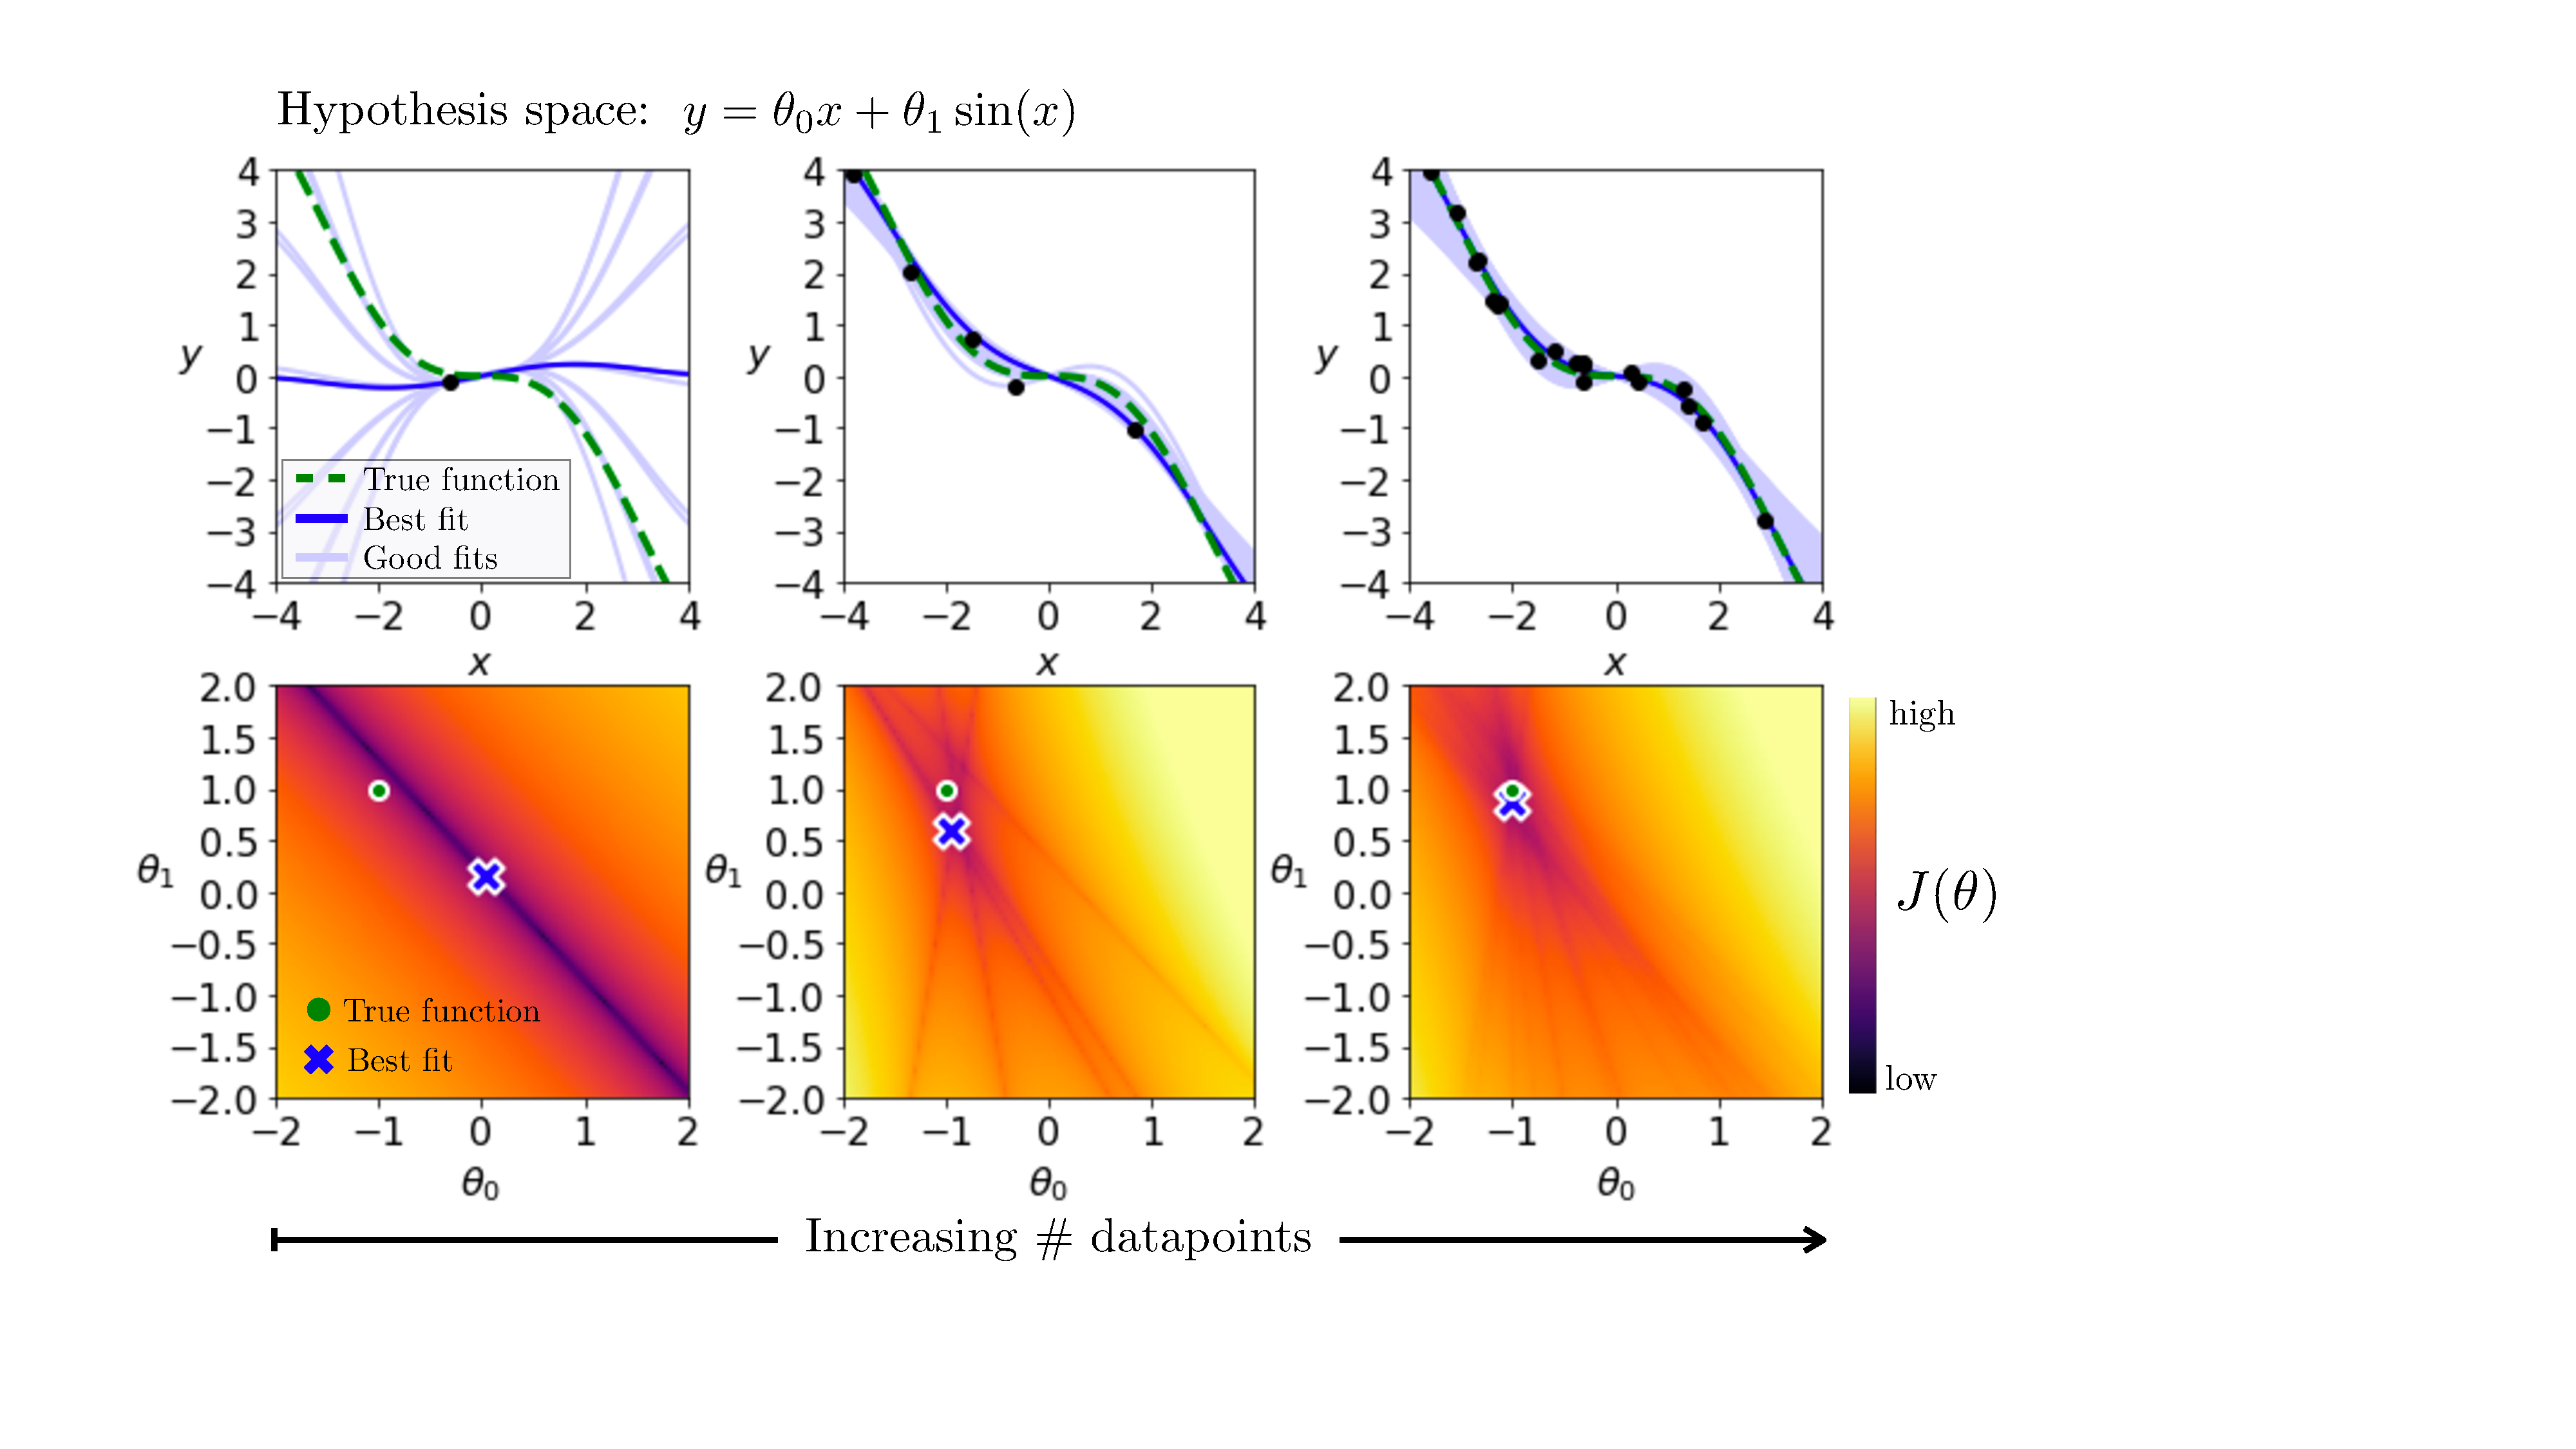
\includegraphics[width=1.0\linewidth]{./figures/problem_of_generalization/more_data_more_constraints.pdf}
    }
    \caption{More data, more (soft) constraints.}
    \label{fig:problem_of_generalization:more_data_more_constraints}
\end{figure}
\marginnote{The heatmaps here are reminiscent of a classic computer vision algorithm called the Hough transform~\cite{hough1959machine,duda1972use}. This transform can be used to find geometric primitives that fit feature points in images. In fact, the bottom row is \textit{exactly} the generalized Hough transform~\cite{duda1972use} of the data points in the top row, using $\theta_0 x + \theta_1 \sin(x)$ as the family of geometric primitives we are fitting.}[-9cm]

The first thing to look at is the leftmost column, where $N=1$. For a single datapoint, there are an infinite number of functions in our hypothesis space that perfectly fit that point. This shows up in the heatmaps as a \textit{line} of settings of $\theta$ that all achieve zero loss.\marginnote{Why a line? Because we have \textit{two} free parameters, $[\theta_0, \theta_1]$, and \textit{one} constraint, $y^{(1)} = \theta_0 x^{(1)} + \theta_1 \sin(x^{(1)})$, so we have one more parameter than constraint yielding a one-dimensional (1D) subspace of solutions.}[-0.4cm] The learning algorithm we used in this example picks a random solution from the set of solutions that achieve zero loss. Unfortunately, here it got unlucky and picked a solution that happens to be far from the true solution.

Next, look at the second column where we have $N=5$ training points. Ideally we want to find a curve that exactly passes through each point. Each \textit{single} datapoint adds one constraint to this problem, and each constraint shows up as a line in the heatmap for $J$ [the line of solutions that satisfy the constraint $y^{(i)} = \theta_0 x^{(i)} + \theta_1 \sin(x^{(i)})$ for that datapoint $i$]. The \textit{intersection} of all these constraints pinpoints the setting of parameters that fits \textit{all} that data. In this example, with five datapoints, there is no location where all the constraint lines intersect, which means there is no curve in our hypothesis space that can perfectly fit this data. Instead we settle for the curve that best approximates the data, according to our loss function. Notice that the learned solution is now pretty close to the true function that generated the data. It is not an exact match, because the data is generated by taking \textit{noisy} samples from the true data generating function.

Finally, let's look at the third column, where we are fitting 20 datapoints. Now the intersection (or, more precisely, average) of the losses for all the datapoints gives a relatively smooth cost function $J(\theta)$, and the learned solution is almost right on top of the true solution. This illustrates a very important point:
\begin{center}
    \textit{The more data you have, the less you need other modeling tools.}
\end{center}%\marginnote{As long as 1) the truth is within the hypothesis space, 2) the noise level is finite, and 3) what you care about is inferring truth.}

With enough data, the true solution will be pinpointed by data alone. However, when we don't have enough data, or when the data is noisy or incorrectly labeled, we can turn to our two other tools, which we will see next.
% processing is too expensive

%This point has several implications that are good to keep in mind. First, generally, the more data you have the better. Second, the more data you have, the less you need other tools to identify the truth -- if you have enough data you don't need regularizers or constraints. Third, because data scale tends to increase over time (we have more and can process more), you should expect that whatever architecture/regularizers are used in year $X$, a less constrained architecture with less regularized will be preferred in year $Y$, for $Y>X$. This is a rule of thumb that has been borne time and again: whatever \textit{inference} methods you learn in this book (meaning optimizers, features, objectives, architectures, models, etc), expect that fewer and fewer of them will be relevant in each subsequent year. Not because new methods will come along that make the current ones out of date (yes that will happen too) but because fewer and fewer methods are useful as data and compute scale. In some year $Z$ we will have enough data and compute that very ``naive'' methods are just as effective as the most sophisticated present approaches. This idea has been called ``the bitter lesson'' and it's good to get comfortable with it now so that you won't have a bitter surprise in a few years. 


\subsection{Experiment 2: Effect of Priors}

Now we will run a similar experiment to look at the effect of priors. In this experiment we will use a slightly different hypothesis space and objective function, namely
\begin{align}
    J(\theta; \{x^{(i)}, y^{(i)}\}^N_{i=1}) &= \frac{1}{N}\sum_i \norm{f_{\theta}(x^{(i)}) - y^{(i)}}_2^2 + \lambda \norm{\theta}_2^2 \quad\quad \triangleleft \quad\text{objective}\\
    f_{\theta}(x) &= \theta_0 x + \theta_1 x \quad\quad \triangleleft \quad\text{hypothesis space}
\end{align}
We will look at the effect of the ridge regularizer $\norm{\theta}_2^2$. We plot the energy landscape and function fit for this problem in \fig{\ref{fig:problem_of_generalization:more_regularizer_more_constraints}}, fitting to a single datapoint. The ridge regularizer prefers solutions with small parameter norm, so its contribution to the energy landscape is to place a quadratic bowl around the origin. As we increase $\lambda$ (moving left to right in the subplots), the effect of the regularizer becomes stronger and pulls the learned solution closer and closer to the origin.

\begin{figure}[t]
    \centerline{
    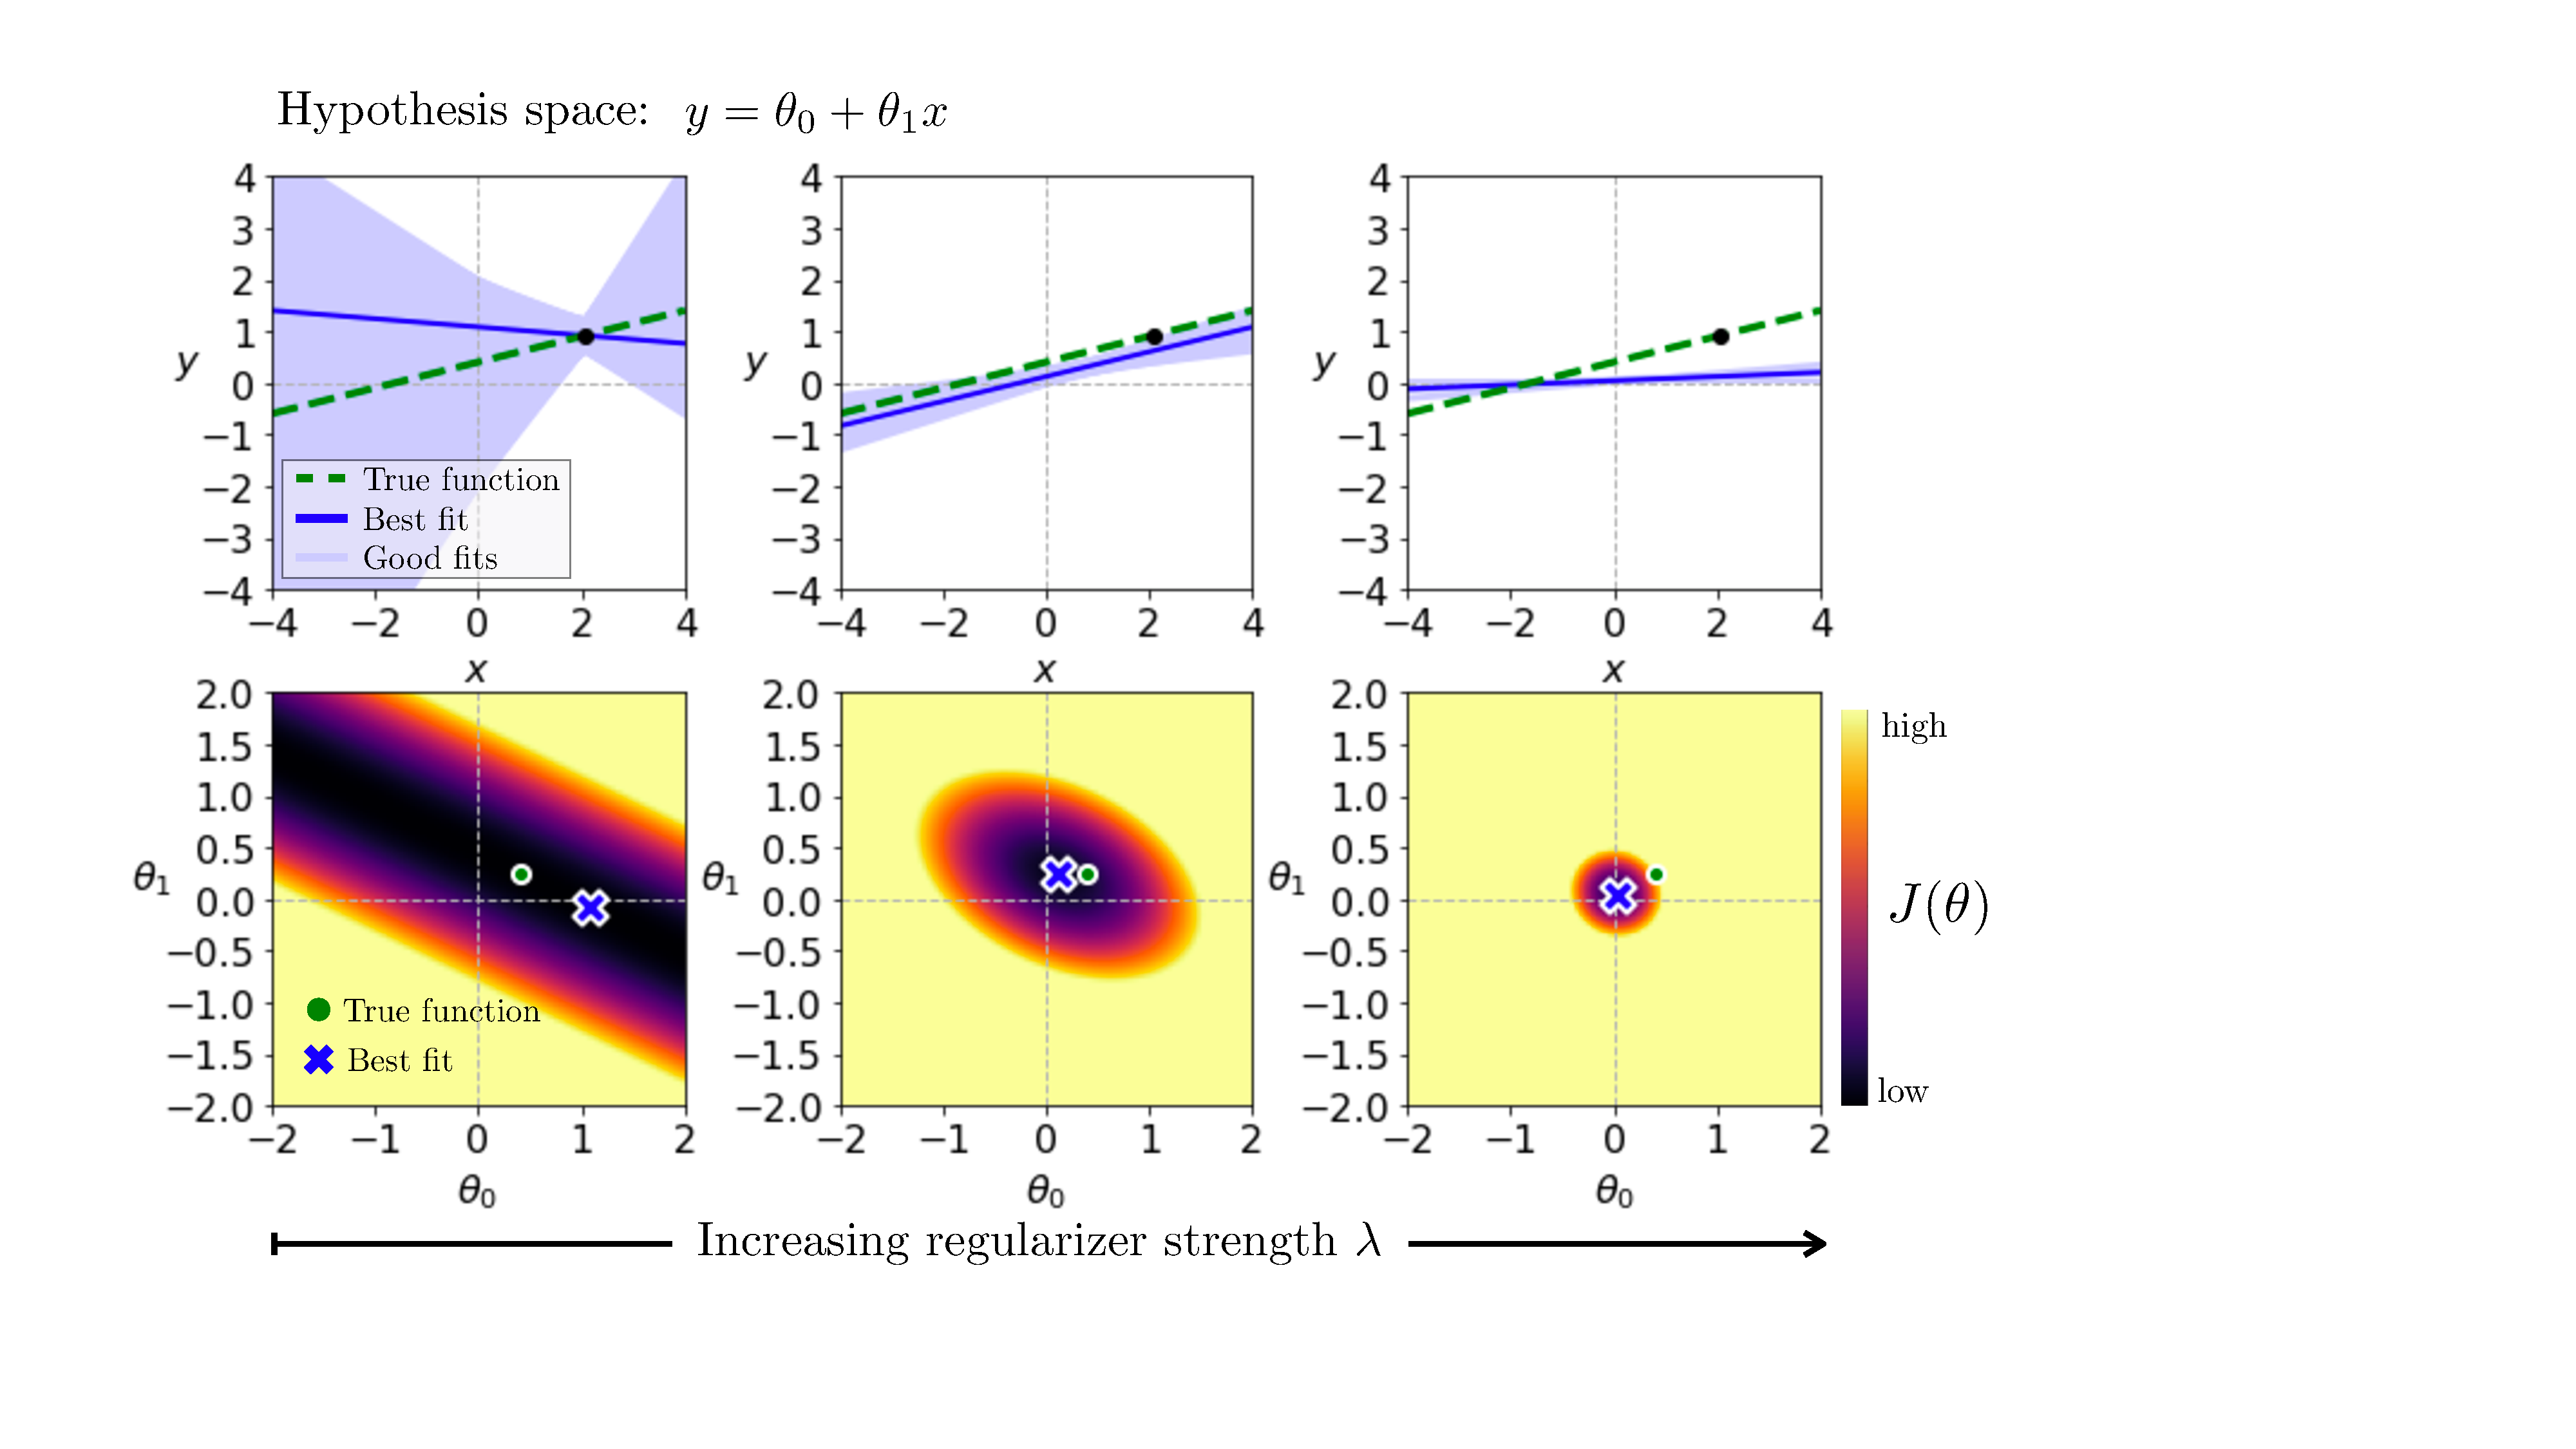
\includegraphics[width=1.0\linewidth]{./figures/problem_of_generalization/more_regularizer_more_constraints.pdf}
    }
    \caption{More regularization, more (soft) constraints.}
    \label{fig:problem_of_generalization:more_regularizer_more_constraints}
\end{figure}

In this example, the true solution lies near the origin, so adding some regularization gets us closer to the truth. But using too strong a $\lambda$ overregularizers; the true solution is not \textit{exactly} $\theta=0$. The middle column is the Goldilocks solution, where the strength of the regularizer is just right.

You can take away a few lessons from this example:
\begin{enumerate}
    \item Priors help only when they are good guesses as to the truth.
    \item Overreliance on the prior means ignoring the data, and this is generally a bad thing.
    \item For any given prior, there is a sweet spot where the strength is optimal. Sometimes this ideal strength can be derived from modeling assumptions and other times you may need to tune it as a hyperparameter.
\end{enumerate}

\subsection{Experiment 3: Effect of the Hypothesis Space}

Now we turn to the last of our tools: the hypothesis space itself. For this experiment, we will use the same objective as in \eqn{\ref{eqn:problem_of_generalization:error_fn_1}} and we will consider the following three hypothesis spaces:
\begin{align}
    f_{\theta}(x) &= \theta_0 x + \theta_1 x^2 &\triangleleft \quad\texttt{quadratic}\\
    f_{\theta}(x) &= \theta_0 x &\triangleleft \quad\texttt{linear}\\
    f_{\theta}(x) &= 0 &\triangleleft \quad\texttt{constant}
\end{align}
Our experiment on these three spaces is shown in \fig{\ref{fig:problem_of_generalization:fewer_hypotheses_more_constraints}}. We show the hypothesis spaces in order of decreasing size moving to the right.

\begin{figure}[t]
    \centerline{
    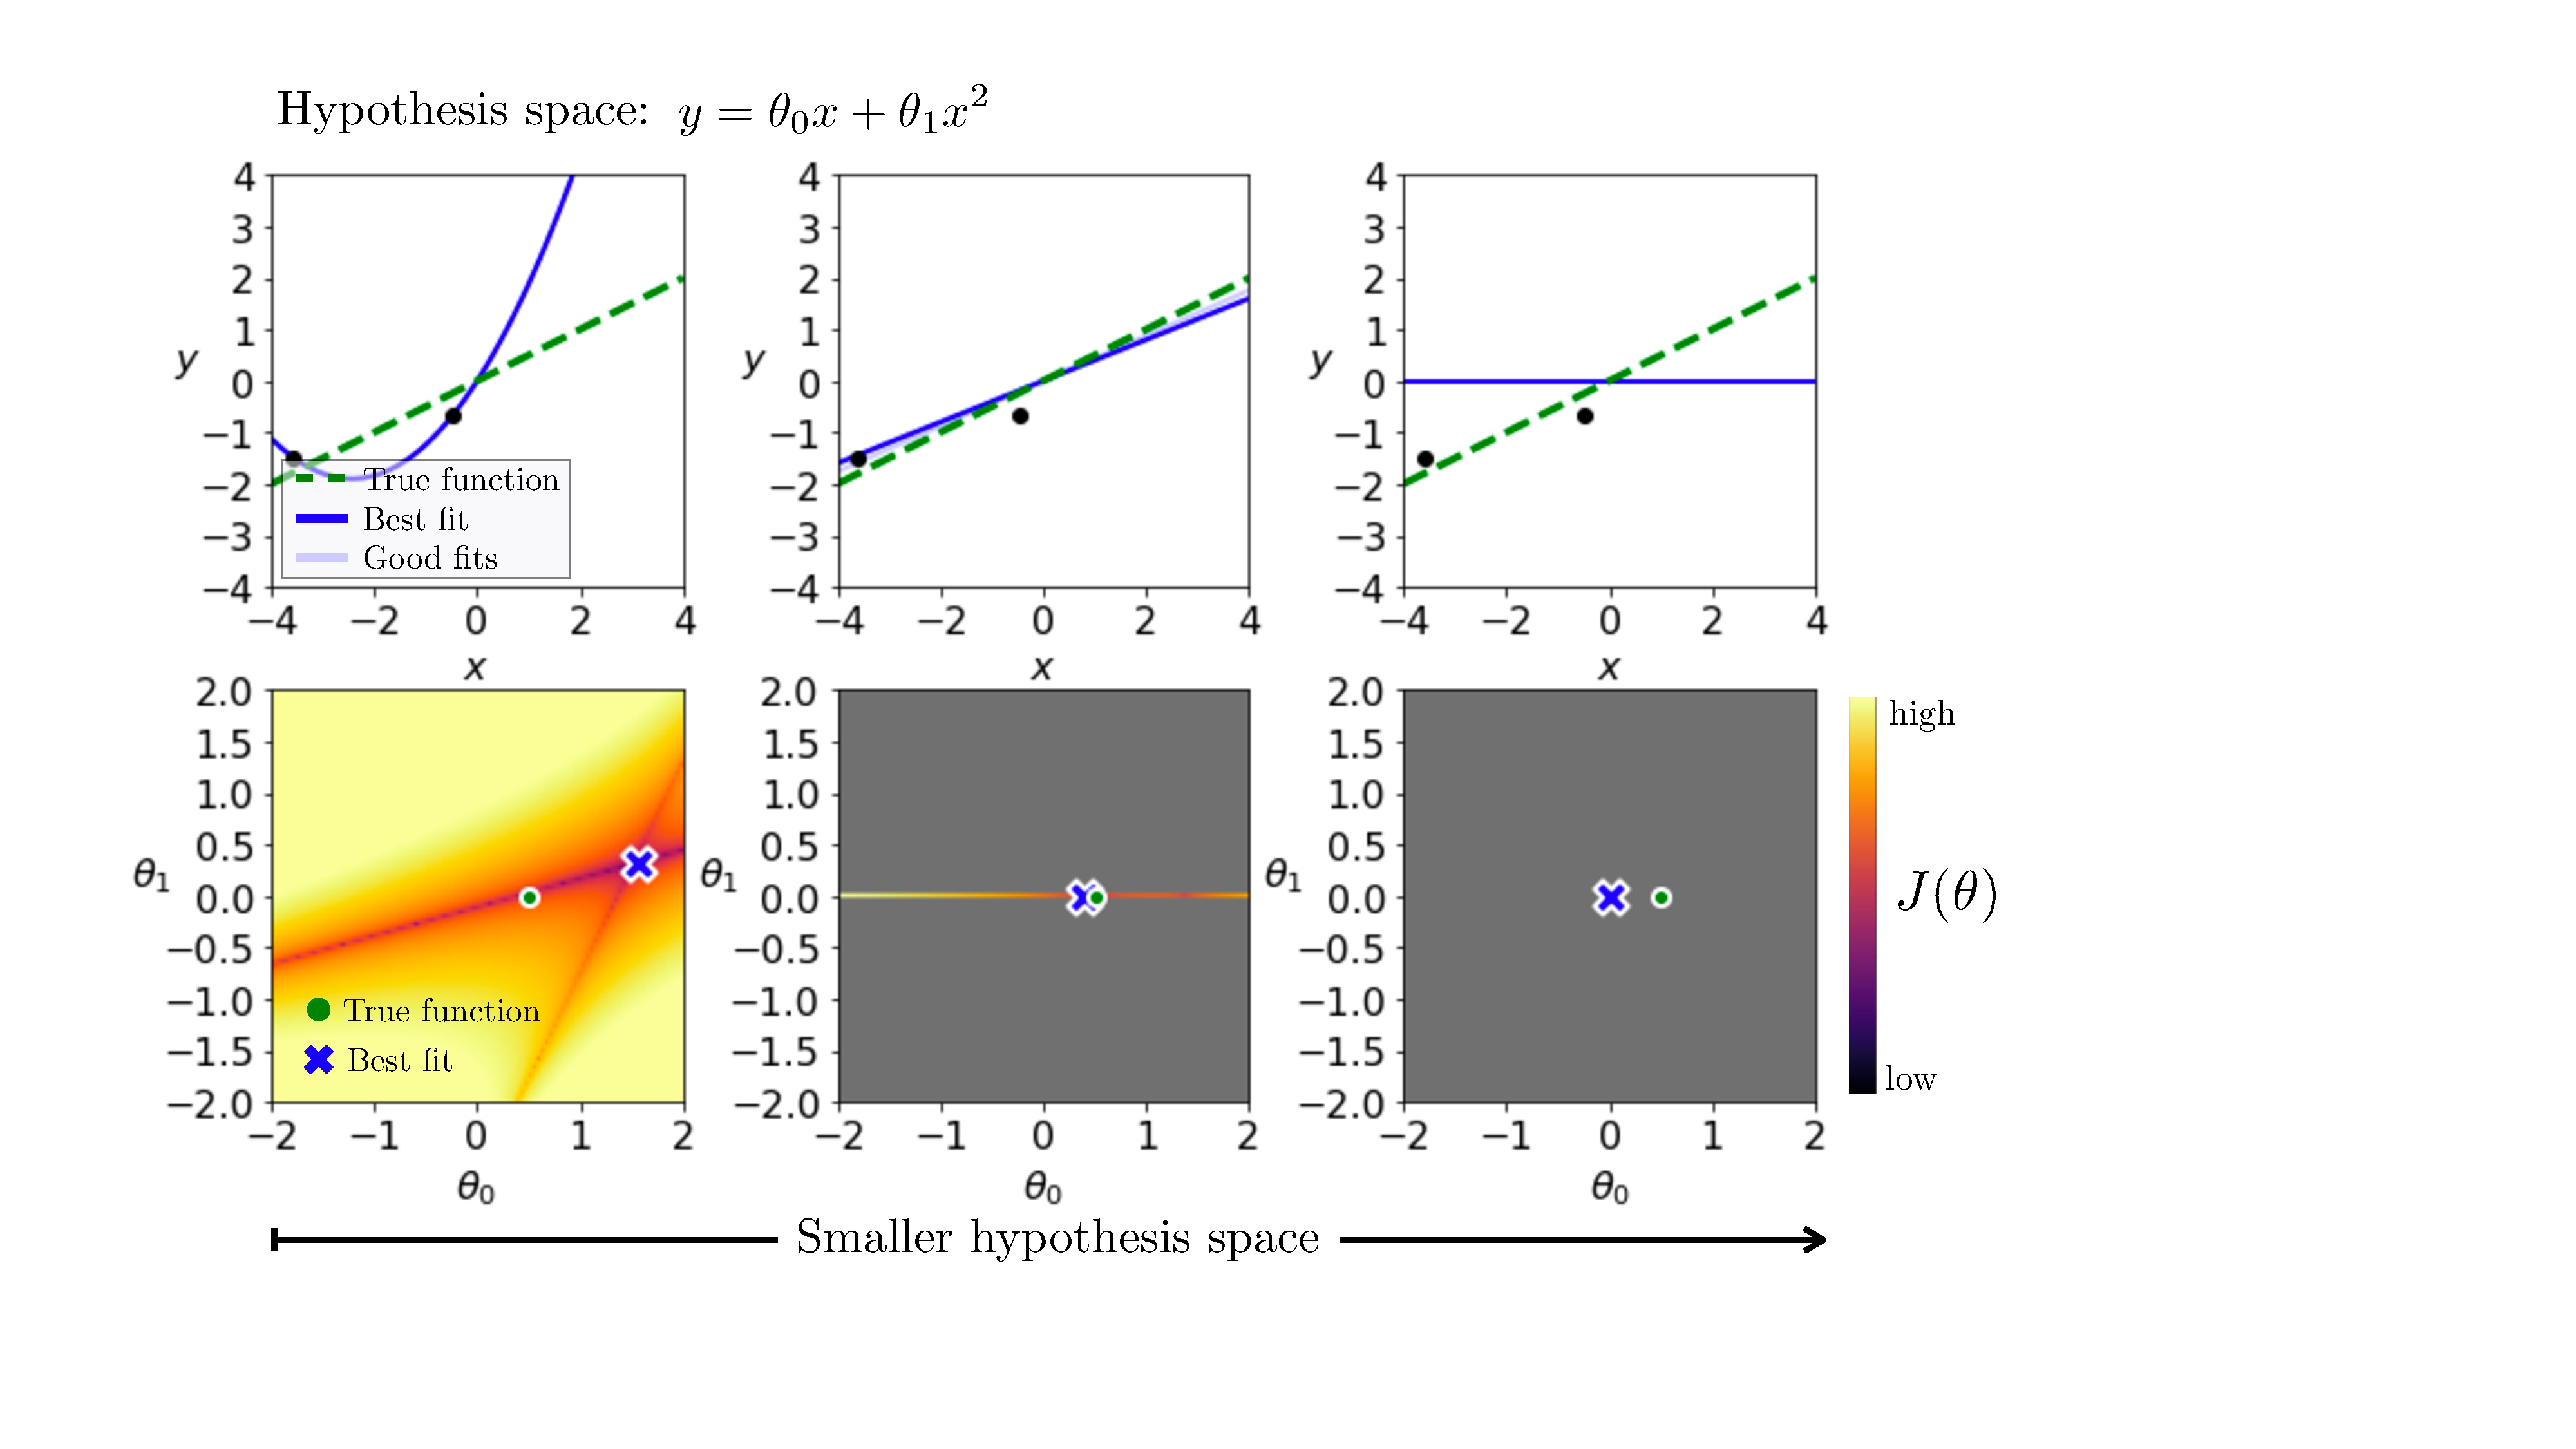
\includegraphics[width=1.0\linewidth]{./figures/problem_of_generalization/fewer_hypotheses_more_constraints.pdf}
    }
    \caption{Fewer hypotheses, more (hard) constraints.}
    \label{fig:problem_of_generalization:fewer_hypotheses_more_constraints}
\end{figure}

The true function is linear, and because of that both the \texttt{quadratic} and \texttt{linear} hypothesis spaces contain the true solution. However, the linear hypothesis space is \textit{much} smaller than the quadratic space. For the linear hypothesis space, searching for the solution (i.e., learning) only considers the slice of parameter space where $\theta_1=0$; all the gray region in \fig{\ref{fig:problem_of_generalization:fewer_hypotheses_more_constraints}} can be ignored. Using a smaller hypothesis space can potentially accelerate our search. %This leads us to a general principle:
%\begin{center}
%    \textit{A smaller hypothesis space can accelerate the search for truth.}
%\end{center}
%\marginnote{Remember, the hypothesis space and parameterization are \textit{not} the same thing (see \chap{\ref{chapter:intro_to_learning}}, \sect{\ref{sec:intro_to_learning:key_ingredients}}). \textit{Overparameterizating} a small hypothesis space can make learning faster.}[-0.4cm]

However, clearly you can go too far, as is demonstrated by the \texttt{constant} hypothesis space (far right column). This hypothesis space only contains one function, namely $f_{\theta}(x) = 0$. Search is trivial, but the truth is not in this space.

%One important thing to note is that the hypothesis space is not the same as the parameterization. The same hypothesis space can be parameterized in many ways. For example, a linear function $\mathbb{R} \rightarrow \mathbb{R}$ can be parameterized either as $f_{\theta}(x) = \theta_0 x$ or as $f_{\theta}(x) = \theta_1 \theta_0 x$, or as $f_{\theta}(x) = (\theta_1 + \theta_0) x$ or infinite other possiblities, as long as the parameters all end up describing a linear function of $x$. All these parameterizations span the same hypothesis space: linear relationships between $x$ and $y$. You might be tempted to think that fewer parameters is better, since a smaller hypothesis space is generally better (as long as it contains the truth). But this is not always the case. \textit{Overparameterized} models, which have more parameters than the minimum necessary to describe the hypothesis space, sometimes confer benefits in terms of implicit regularization and optimization speed~\cite{XX}. The virtues of overparameterization are being actively studied in the context of deep neural nets (which are generally highly overparameterized)~\cite{XX}.

\subsection{Summary of the Experiments}

These three experiments demonstrate that data, priors, and hypotheses can all constrain our search in similar ways. All three rule out some parts of the full space of mappings and help us focus on others. 

This leads us to another general principle:
\begin{center}
    \textit{What can be achieved with any one of our tools can also be achieved with any other.\footnote{However, note that the hypothesis space places \textit{hard} constraints on our search; we cannot violate them. Data and priors apply \textit{soft} constraints; we can violate them but we will pay a penalty.}}
\end{center}
%\marginnote{* However, note that the hypothesis space places \textit{hard} constraints on our search; we cannot violate them. Data and priors apply \textit{soft} constraints; we can violate them but we will pay a penalty.}
If you don't have much data, you can use strong priors and structural constraints instead. If you don't have much domain knowledge, you can collect lots of data instead. This principle was nicely articulated by Ilya Sutskever when he wrote that ``methods ... are extra training data in disguise''~\cite{dataindisguise}. %And we can equally well say: training data is extra methods in disguise.


\section{Concluding Remarks}
The goal of learning is to extract lessons from past data to help on future problem solving. Unless the future is \textit{identical} to the past, this is a problem that requires generalization. One goal of learning algorithms is to make systems that generalize ever better, meaning they continue to work even when the test data is very different than the training data. Currently, however, the systems that generalize in the strongest sense—that work \textit{for all} possible test data—are generally not learned but designed according to other principles. In this way, many classical algorithms still have advantages over the latest learned systems. But this gap is rapidly closing!